In the previous chapter, we described our methodology. We presented the framework we used for our setup, and we went into detail on the configuration of the experiments, and the project as a whole describing both the masking and the neural networks. 
In this chapter, we will start with the description of the datasets used on the results and the metrics chosen as a reference point for the evaluation of our results. 
Finally, for each model, we will evaluate it for the datasets we have presented.

\section{Datasets}
To show and explain the experiments, we need to look at the datasets we have to evaluate our results. 
\todo{something about Simula already researching on this}

In this thesis, we primarily use four datasets to train and evaluate our results.

\iffalse

\subsection{kvasir}


As we recall from the introduction chapter, oesophagal, stomach and colorectal cancer accounts for about 2.8 million new cases and 1.8 million deaths per year, and this number is increasing as the population gets older.   With automatic detection of diseases by use of computers being prominent, but a still unexplored field of research the dataset Kvasir was made.
Kvasir is a Multi-Class Image Dataset for Computer Aided Gastrointestinal Disease Detection made in Norway. The data is gathered from the Vestre Viken Health Trust, and it contains not only polyps but also two other findings, two classes related to polyp removal and three anatomical landmarks in the GI tract.

The data is collected using endoscopic equipment at Vestre Viken Health Trust in Norway. The Vestre Viken Health Trust is a collection of 4 hospitals, and it provides health care to 470.000 people.
One of the more prominent hospitals in this group is Bærum Hospital. It has a large gastroenterology department where the data originates, and more data will be provided in the future. The data from Bærum Hospital has been annotated by medical experts and the Cancer Registry of Norway before its inclusion in the Kvasir dataset, making the data thoroughly marked and checked.
The Cancer Registry of Norway work provides new knowledge about cancer prevention and cancer treatment. It is part of the South-Eastern Norway Regional Health Authority and organised as an independent institution under Oslo University Hospital Trust. The Cancer Registry of Norway is responsible for the national cancer screening programmes with the goal to ultimately prevent cancer death by discovering cancers or pre-cancerous lesions as early as possible. 

\cite{runeMedico2018}

Kvasir is a dataset containing images from inside the gastrointestinal tract containing three anatomical landmarks, in the form of the Z-line (a), the Pylorus (b) and the Cecum (c). Also, the Kvasir dataset includes two categories of images related to endoscopic polyp removal, Dyed and Lifted Polyps (d) and Dyed Resection Margins (e), and lastly, three classes, Esophagitis (g), Polyps (h), and Ulcerative Colitis (i), containing images of pathological findings.


\subsubsection{Anatomical Landmarks}
The definition of an anatomical landmark is a feature that is easily recognisable through an endoscope. For the medical staff they are essential for navigating the GI tract, and the assist as a reference point both for a physical location, and to describe the position for a relevant finding.
It is often relevant for a complete endoscopic report to contain image documentation and a description of these three landmarks.
 
\paragraph{Z-line}
The Z-line is the sphincter between the oesophagus and the stomach. This sphincter is an endoscopically recognisable border where the white mucosa meets the red gastric mucosa from the stomach.  When performing endoscopy an assessment of the Z-line is important to determine whether disease is present or not. A malfunctioning sphincter can, for instance, lead to diseases like gastroesophageal reflux. \todo{cite}.
Figure \ref{fig:z-line} shows a normal z-line taken from an endoscopy. 

\textbf{Pylorus}
We call the barrier between the stomach and the upper part of the small bowel for the Pylorus. This sphincter is responsible for letting food from the stomach into the GI tract, and to keep the stomach acid from flowing into the bowels.
Medical staff inspect both sides of the pylorus when doing a complete colonoscopy and endoscopy. This inspection is crucial to identify findings like ulcerations, erosions or stenosis.  \todo{cite}
Figure \ref{fig:pylorus} shows an endoscopic image of a healthy pylorus taken from inside the stomach.

\textbf{Cecum}
The last anatomical landmark used in gastronomy is the cecum. It is an intraperitoneal pouch that is considered to be the beginning of the large intestine. This area in the GI tract is considered the final stop for a standard colonoscopy as it is the last quality indicator for the procedure.
Being the last landmark, the identification and inspection of this area are one of the most crucial steps in the whole inspection. 
Figure \ref{fig:cecum} shows a normal cecum.


\subsection{Pathological Findings}
Pathological findings are areas or objects with an abnormal or unwanted feature. When looking at it from the oral entrance, pathological findings takes the form of inflammation, while in the lower GI tract it takes the form of, for instance, polyps. 
Pathological findings are the group of images that are especially important to detect and classify as they impose the most significant risk for the patients well being. \todo{do not like the ending}


\paragraph{Esophagitis}
Esophagitis is an inflammation oesophagus near the Z-line. Usually, the oesophagus is composed of a mucosal lining and circular smooth muscle fibres, but when a patient has a condition like a gastroesophageal reflux disease the area can become inflamed. 
Clinically, detection of this inflammation is necessary for treatment initiation to relieve the symptoms and to prevent further development that can lead to more complications.


\paragraph{Polyps}
Polyps are lesions in the bowel detectable as mucosal outgrowths. There are multiple types of polyps that are either flat, elevated, or pedunculated. Polyps are distinguishable from normal mucosa as they have a different colour and surface texture. Most of these bowel anomalies are harmless, but they have, as discussed in the introduction, the possibility to become cancerous. 
There is a big focus dedicated to the removal and detection of there polyps as they are a significant threat to cancer of not treated in time. Because of the different shape and rate of outgrowth, medical staff overlook a small, but significant part of the polyps during routine procedures. 
This rate of error was the most significant driving force for investing in computer-aided medical diagnosis, and subsequently creating the Kvasir dataset.

\paragraph{Ulcerative Colitis}
Ulcerative Colitis is the last pathological finding type in the Kvasir dataset. 
It is a chronic inflammatory disease affecting the large bowel. Ulcerative Colitis may both come from psychological and physiological factors, but the origin of the disease is often unknown. The degree of inflammation is a factor when performing medical diagnosis, though in the Kvasir dataset we only have one class of ulcerative colitis.
A severe example of ulcerative colitis can is seen in figure \ref{fig:ulcerativecolitis}. Here we have an evident inflammation, and thus this would most likely be classified as severe.



\subsection{Polyp Removal}
The last groups are concerned with the removal of polyps. A technique often used in polyp removal is endoscopic mucosal resection (EMR). \todo{cite}
This procedure includes the injection of a liquid underneath the polyp, lifting it from the underlying tissue. After the injection, the medical staff use a snare to wrap around remove the polyp. Using this method of lifting and snaring, the medical staff reduces the risk of damaging the surrounding tissue by a large margin.

\paragraph{Dyed and Lifted Polyps}
The first of the two classes concerning polyp removal is the Dyed and Lifted Polyps class. This case is the polyp after it has been lifted from the surrounding tissue, and the next step is to use a snare to remove it.
Figure \ref{fig:dyedandliftedpolyps} shows a polyp after the injection liquid is applied. 


\paragraph{Dyed Resection Margins}
The resection margin is important to evaluate after the removal of a polyp, as we want to be sure the entirety of the are is clean. 
If the procedure did not eradicate the polyp, the residual polyp tissue might lead to continued growth, and in the worst case malignancy development. 




%\subsection{Nerthus} 
\todo{do we do Nerthus?}
\subsection{CVC-356}
The 

\subsection{CVC-12k}
\subsection{CVC-612}

esdtgfgv

 
    


%============================================

    \begin{figure}[h!]
        \centering
        \begin{subfigure}[b]{0.4\textwidth}
            \centering
            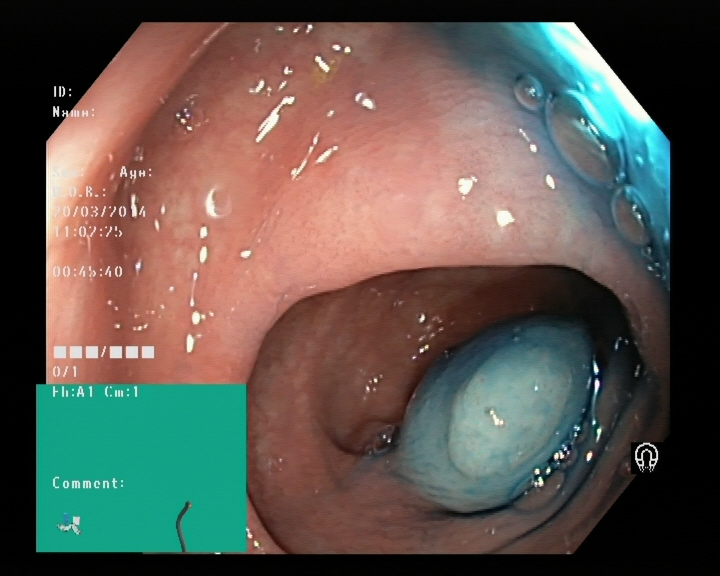
\includegraphics[width=\textwidth]{experiments/images/dyed-lifted-polyps.jpg}
            \caption[Is this in use]%
            {{\small  }}    
            \label{fig:polypAEGREEN}
        \end{subfigure}
        \qquad
        \begin{subfigure}[b]{0.4\textwidth}  
            \centering 
            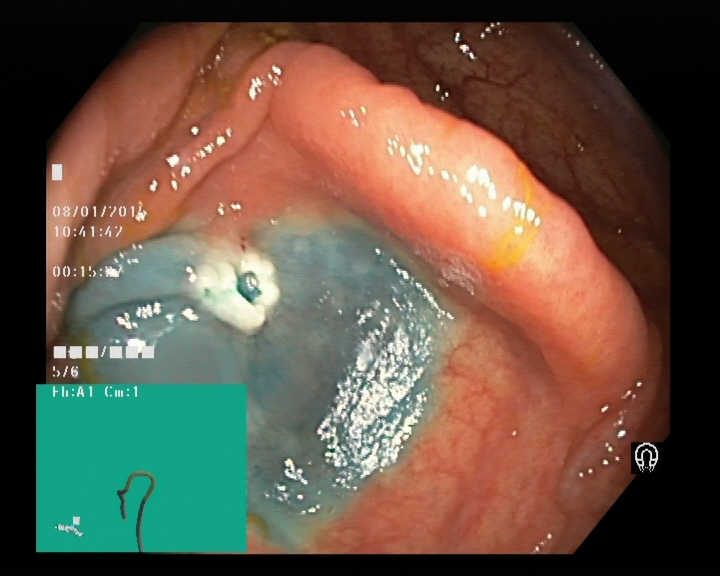
\includegraphics[width=\textwidth]{experiments/images/dyed-resection-margins.jpg}
            \caption[Hate to be this guy]%
            {{\small }}    
            \label{fig:polypGAN}
        \end{subfigure}
        \qquad\vfill%\vskip\baselineskip
        \begin{subfigure}[b]{0.4\textwidth}   
            \centering 
            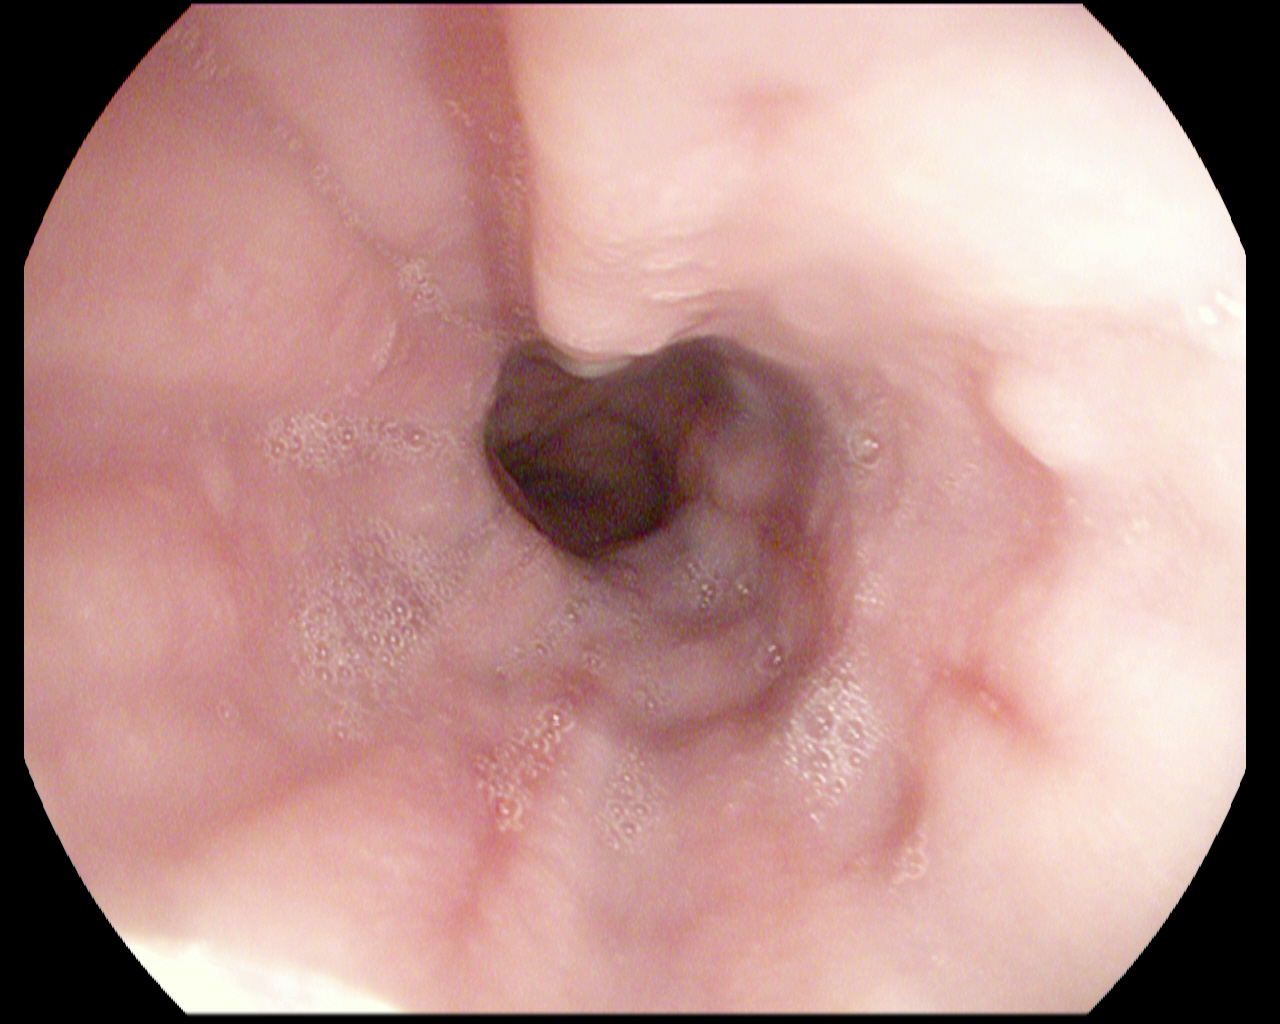
\includegraphics[width=\textwidth]{experiments/images/esophagitis.jpg}
            \caption[]%
            {{\small }}    
            \label{fig:zAE}
        \end{subfigure}
        \qquad%\hfill%\quad
        \begin{subfigure}[b]{0.4\textwidth}   
            \centering 
            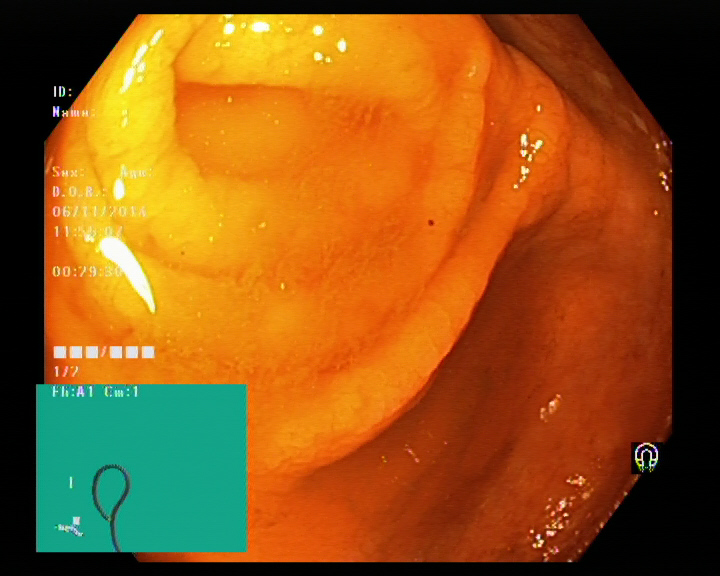
\includegraphics[width=\textwidth]{experiments/images/normal-cecum.jpg}
            \caption[]%
            {{\small }}    
            \label{fig:zGAN}
        \end{subfigure}
        \qquad
        \begin{subfigure}[b]{0.4\textwidth}
            \centering
            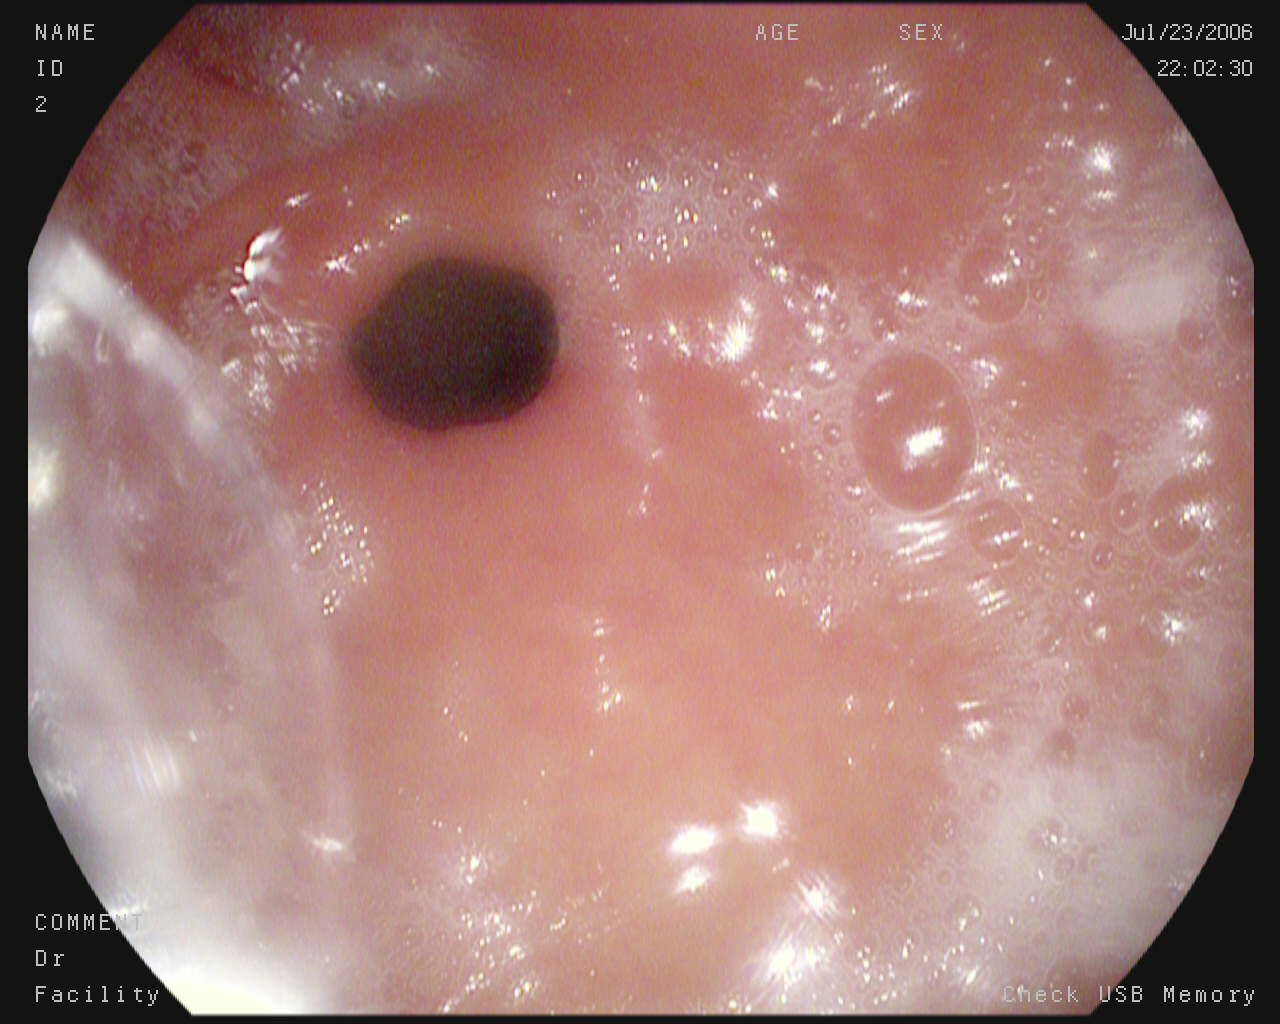
\includegraphics[width=\textwidth]{experiments/images/normal-pylorus.jpg}
            \caption[Is this in use]%
            {{\small  }}    
            \label{fig:polypAEGREEN}
        \end{subfigure}
        \qquad
        \begin{subfigure}[b]{0.4\textwidth}  
            \centering 
            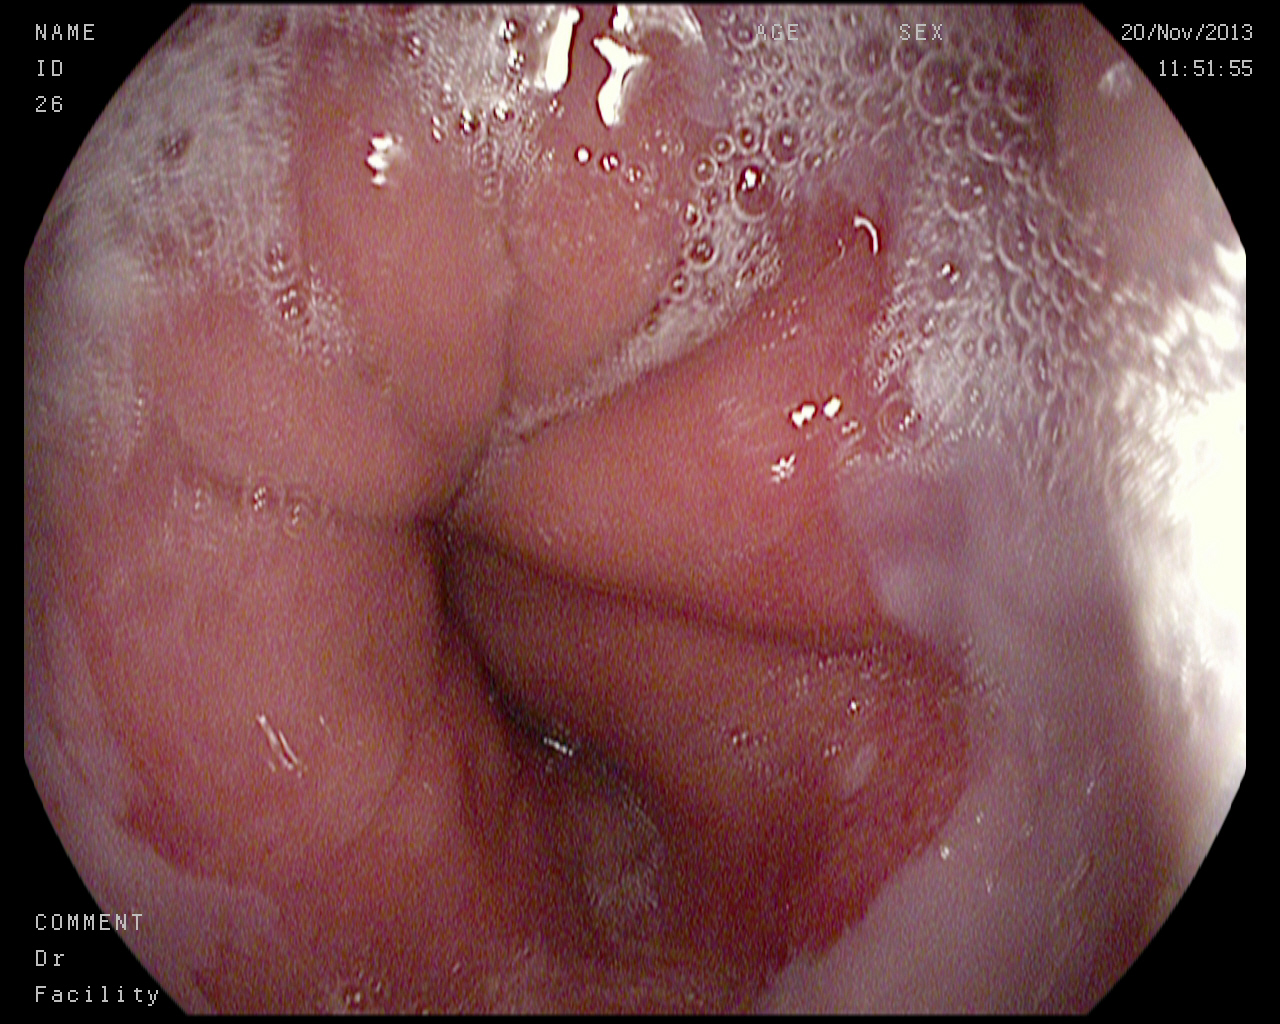
\includegraphics[width=\textwidth]{experiments/images/normal-z-line.jpg}
            \caption[Hate to be this guy]%
            {{\small }}    
            \label{fig:polypGAN}
        \end{subfigure}
        \qquad\vfill%\vskip\baselineskip
        \begin{subfigure}[b]{0.4\textwidth}   
            \centering 
            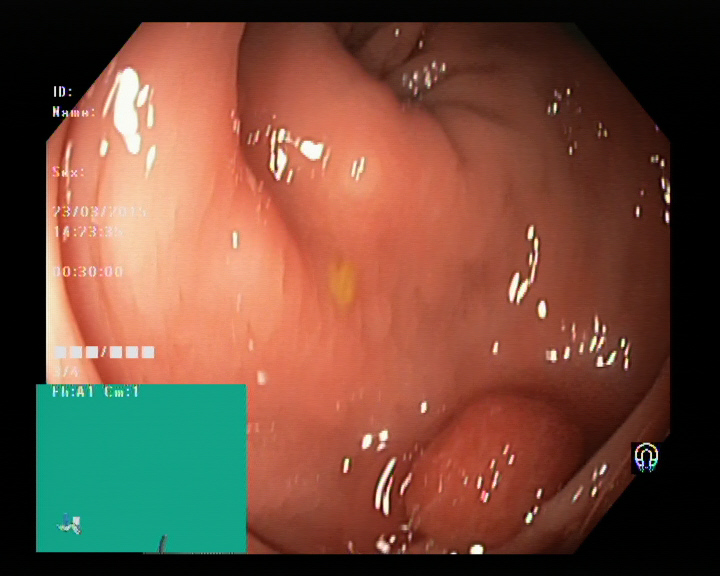
\includegraphics[width=\textwidth]{experiments/images/polyps.jpg}
            \caption[]%
            {{\small }}    
            \label{fig:zAE}
        \end{subfigure}
        \qquad%\hfill%\quad
        \begin{subfigure}[b]{0.4\textwidth}   
            \centering 
            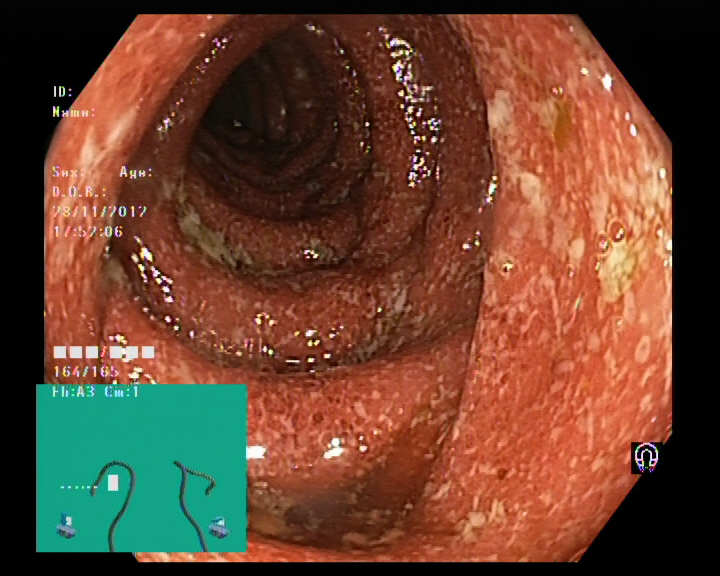
\includegraphics[width=\textwidth]{experiments/images/ulcerative-colitis.jpg}
            \caption[]%
            {{\small }}    
            \label{fig:zGAN}
        \end{subfigure}
        \caption[ ]
        {\small New text here} 
        \label{fig:GC1GREEN}
    \end{figure}
    
   
\FloatBarrier


    %=============================================
\fi
\section{Metrics}
To discern the results of our experiments we introduce multiple metrics and tables to get an indication of our success. 
The main dataset we used for training, Kvasir, was split into k number of folds, using k-fold cross-validation. 
K-fold cross-validation is a tool used in statistics and machine learning to help to get an accurate representation of the data based on finding a statistical average of the dataset.  In machine learning, it is a powerful tool that can help with adapting to new datasets and prevent overfitting. 
We recall that the Kvasir dataset contains 8000 images, with 1000 of each class. 
In our testing we split the dataset up in k=6 folds. This means that we split our dataset into six pieces before training.  With the six folds, we assign one of them as a test set, and we assign the four other for training and validation. We then train our data five times, using four folds for training and the last fold for validation during training. For each training run we rotate the validation set, so each of the five folds is used for validation once. \todo{img of k fold}

\begin{figure}[h]
\hspace*{-1cm}                                                           
\centering
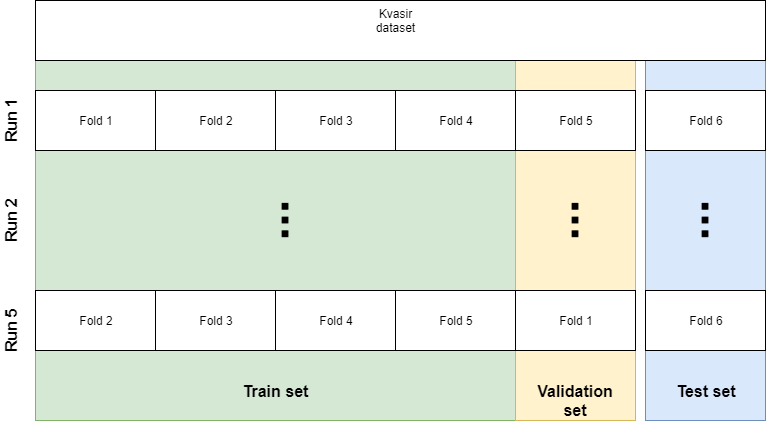
\includegraphics[scale=0.4]{experiments/figures/KfoldKvasir_compressed.png}
\caption{The Kvasir divided in to 6 folds}
\label{fig:KfoldKvasir}
\end{figure}

The advantage of this method is that we maximise the utility of the dataset. We find the distribution of the dataset that hopefully covers the most significant range of the unseen data. 

\subsection{Presentation of data, confusion matrix}
With k-fold cross-validation, we end up with the dataset that scored the highest during the final validation step.  There are multiple ways to calculate metrics for how well a dataset is doing,  but they all are a comparison of the predicted class versus the true class.  
%A:dyed-lifted-polyps , B:dyed-resection-margins , C:esophagitis , D:normal-cecum , E:normal-pylorus , F:normal-z-line , G:polyps , H:ulcerative-colitis , I:non-polyp

Take for instance the case with the 8-class dataset Kvasir, where we predict an image to be normal-cecum. We translate this to an integer representation of, for instance, class 3. In our example the actual True class is normal-z-line, here represented as 5. 

We can represent this as 
\[
\begin{bmatrix}
 3 & 5\\ 
\end{bmatrix}
\]
Storing value pairs like this can very quickly get cluttered and unorganised.
The most common way to store these value pairs is to use a confusion matrix.  We initiate the matrix as a \textit{$N \times N$} matrix where N is the total number of classes as shown in Figure \ref{mat:emptyCM}

\begin{figure}
    \centering
    \[
    \begin{bmatrix}
     0 & 0 &  0 &  0 &  0 &  0 &  0 &  0\\
     0 & 0 &  0 &  0 &  0 &  0 &  0 &  0\\
     0 & 0 &  0 &  0 &  0 &  0 &  0 &  0\\
     0 & 0 &  0 &  0 &  0 &  0 &  0 &  0\\
     0 & 0 &  0 &  0 &  0 &  0 &  0 &  0\\
     0 & 0 &  0 &  0 &  0 &  0 &  0 &  0\\
     0 & 0 &  0 &  0 &  0 &  0 &  0 &  0\\
     0 & 0 &  0 &  0 &  0 &  0 &  0 &  0\\
    \end{bmatrix}
    \]
    \caption{An empty confusion matrix}
    \label{mat:emptyCM}
\end{figure}



After we have initialised the confusion matrix, we add each value pair as to the matrix at is corresponding position.  
Given the pair $\begin{bmatrix} 3 & 5 \end{bmatrix}$ we add one to the position corresponding to (x=3,y=5). 
 Another example could be given the pair where we guessed class 0 and the true class was 0:  $\begin{bmatrix}  0 & 0 \end{bmatrix}$, we add one to the matrix at position (x=0,y=0). Witch 2 examples we get the following confusion matrix shown in Figure \ref{mat:nonemptyCM}

\begin{figure}
    \centering
    \[
    \begin{bmatrix}
     1 & 0 &  0 &  0 &  0 &  0 &  0 &  0\\
     0 & 0 &  0 &  0 &  0 &  0 &  0 &  0\\
     0 & 0 &  0 &  0 &  0 &  0 &  0 &  0\\
     0 & 0 &  0 &  0 &  0 &  0 &  0 &  0\\
     0 & 0 &  0 &  0 &  0 &  0 &  0 &  0\\
     0 & 0 &  0 &  1 &  0 &  0 &  0 &  0\\
     0 & 0 &  0 &  0 &  0 &  0 &  0 &  0\\
     0 & 0 &  0 &  0 &  0 &  0 &  0 &  0\\
    \end{bmatrix}
    \]
    \caption{The confusion matrix with [3 5] and [0 0] inserted }
    \label{mat:nonemptyCM}
\end{figure}

As we fill in the matrix with more predictions we can start to draw conclusions from it. After approximately 1600 evaluations, our result might at the end look like this.
\begin{figure}
    \centering
    \[
    \begin{bmatrix}
     195 & 50 &  0 &  0 &  0 &  0 &  2  & 1\\
       4 & 148&  1 &  0 &  0 &  0 &  0  & 0\\
       0 &  0 & 152&  0 &  3 & 40 &  0  & 5\\
       0 &  1 &  0 &198 &  0 &  0 & 13  & 4\\
       0 &  0 &  0 & 0  &195 &  1 &  5  & 2\\
       0 &  0 & 47 & 0  &  1 &159 &  0  & 0\\
       1 &  0 &  0 & 0  &  0 &  0 & 172 &  8\\
       0 &  1 &  0 & 2  &  1 &  0 &  8  & 180\\
    \end{bmatrix}
    \]
    \caption{The confusion matrix with  almost 1600 predictions}
    \label{mat:FullCM}
\end{figure}
We can see that the majority of predictions lie around the diagonal. This centralisation means that most of our results were classified correctly, as values at the diagonal are the same x and y values, and subsequently a correct prediction. 
We can also discern something about the four primary metrics associated with a value in the matrix.\\

\textbf{True Positive (TP): } True positive for a specific class is when it is predicted positive, and the True label is also positive.  In the Kvasir dataset, we have a True positive result if, for the class polyp, we predict a polyp.\\

\textbf{True Negative (TN): } True Negative is the opposite of true positive. Given the class Polyp from the Kvasir dataset, we guess that the image is not a polyp when the True label is non-polyp. 

\textbf{False Positive (FP): } False positive is, given a True label we predict False. We often call this type of error a "Type 1 error".   In the polyp case, this is the case where we predict a polyp given no polyp present.


\textbf{False Negative (FN): } False positive is the case where we fail to predict the class when it is True. This type of error is often called "Type 2 error". False Negative is, in our case, the least desirable outcome for our classes with pathological findings like Esophagitis, Polyps and Ulcerative Colitis.

For our multiclass confusion table, we can look at the four metrics like this
\begin{figure}[h]
\centering
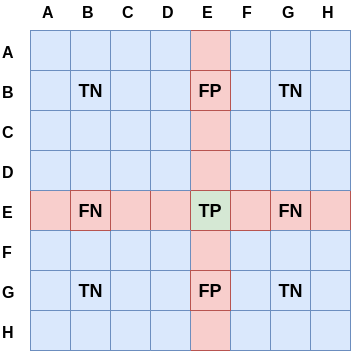
\includegraphics[scale=0.7]{experiments/figures/confusionmatrix.png}
\caption{
Confusion matrix with eight classes, here True positive is marked in green, False Negative and False positive marked in red, and True negative in blue.
}
\label{fig:confusionmatrix}
\end{figure}


\subsection{common Metrics}
When evaluating our results, we use a set of common metrics used in the field of statistics and machine learning.  The metrics we will be using in this thesis are Recall (REC), Precision (PREC), Specificity (SPEC), Accuracy (ACC), Matthews correlation coefficient (MCC), and F1 score (F1). 


\vspace{5px}
\textbf{Accuracy:}  
Accuracy is simply the percentage of the predictions that were classified correctly.
It describes how many of our predictions were correct out of the total predictions made as shown in equation \ref{eq:ACC}. It is the most common metric given its simplicity both in calculation and understanding. 
In general when our data is balanced, and we only have a few classes, we can get away with using accuracy.
A pitfall with accuracy is the lack of comprehensive overview of the data, as it is just a summation without respect to classes involved.
In this project, we use accuracy during the training step as a metric of success. 
 \begin{equation}
ACC=\frac{TP+TN}{TP+TN+FP+FN}
\label{eq:ACC}
\end{equation}

\vspace{5px}
\textbf{Recall:}  
Recall is the probability of detection, or sensitivity.
This metric is a measure of the fraction of relevant instances that have been retrieved over the total amount of relevant instances for a binary classification example.
For our medical image classification, this metric can help us understand how our algorithms work by looking at classes where we have small anomalies in the images, like the case with polyps.
%\todo{ "Detector Performance Analysis Using ROC Curves – MATLAB & Simulink Example". www.mathworks.com. Retrieved 11 August 2016.}

\begin{equation}
REC=\frac{TP}{TP+FN}
\label{eq:REC}
\end{equation}




\vspace{5px}
\textbf{Specificity:} Specificity measures the proportions of our samples that were correctly identified as negative, when the true class were also negative. 
Specificity is related to recall as an opposite in the binary class example.
Equation \ref{eq:SPEC} shows the equation used for specificity.
\begin{equation}
TPR=\frac{TN}{TN+FP}
\label{eq:SPEC}
\end{equation}



\vspace{5px}
\textbf{Precision:}
Precicion is the meassure of relevance in the binary classification case.
As we can see from equation \ref{eq:PREC} the formula is similar to recall, but it only looks at the positive samples. 
\begin{equation}
PREC=\frac{TP}{TP+FP}
\label{eq:PREC}
\end{equation}



\vspace{5px}
\textbf{F1 score:}
F1 score is a combination of precision and recall. It is one of the most common metric to compare the performance of statistical models.
Equation \ref{eq:F1} shows the F1 score as it is most commonly used.

\begin{equation}
F1=\frac{precision \times recall}{precision + recall}
\label{eq:F1}
\end{equation}



\vspace{5px}
\textbf{Matthews correlation coefficient:}
Matthews correlation coefficient is a metric that takes all four possible states of TP, TN, FN and FP in to account. As with the F1 score, the Matthews correlation coefficient gives a score that is based on a more complete understanding of the data compared to how metrics like recall and precision only looks at a subset of the data.

Equation \ref{eq:MCC} shows the formula. It can output a score from -1 to 1, where 1 is a correct classification and -1 a total incorrect prediction. A score of 0 shows no statistical relevance in the result we have.
\begin{equation}
MCC=\frac{TP \times TN - FP \times FN}{\sqrt{(TP + FP)(TP + FN)(TN + FP)(TN + FN)}}
\label{eq:MCC}
\end{equation}







\subsection{Singleclass vs Multiclass Metrics}

The metrics presented are, in general, a solid way to present the validity of a model. However, not all metrics presented is the same when switching between single and multiclass classification.  Metrics like Accuracy is designed to work for multiclass classification, given that there is only one way to calculate the score.
\begin{equation}
\frac{\sum (diag(Covarience Matrix))}{\sum(Covariance Matrix)}
\label{eq:ACCalt}
\end{equation}

The problem with multiclass metrics arises when there is more than one way to calculate the metrics needed, this can be for instance Recall and Specificity, where we have multiple ways to add together the class-wise scores. The three most common ways to calculate the average are:

\textbf{Micro average}: calculates the mean value of each of the binary metrics and averages the result over the total number of samples. 
Micro average ignores all class frequencies and gives us a metric based on all samples gathered. Micro-averaging may be preferred in multilabel settings, including multiclass classification where a majority class is to be ignored.\\

\textbf{Macro average}: calculates the mean of each of the binary metrics, giving the same weight to each of the classes. Macro average gives importance to classes with few samples, and infrequent classes play the same roles as frequent ones. The disadvantage with Macro average is the fact that in the real world some classes often plays a more significant role than others, and doing especially bad on one of the classes can worsen the total result. \\

\textbf{Weighted average} calculates the mean of each of the binary metrics but gives a weighted sum for each of the scores before it is averaged. 
The weight of each class depends on the size of the true data samples.
The weighted average gives us the advantage that small classes still count more than it would with for instance Micro average, but since it depends on the number of samples from each class it can end up more or less as a black box during calculation.
Weighted average gives us the best of both worlds, but it lacks the intuitiveness from the two other classes. \\

With the three methods presented, we have chosen to Macro average our results. While both Macro and Weighted average would give a good indication given that not all our datasets are balanced, we argue that the weighted average would give metrics that are harder to explain when we are working on datasets with unbalanced classes.

In addition to looking at the Macro average of precision and recall, we want to look at specific cases of the classification.  In many cases, we have multiple classes, where we are most interested in just one or a handful of the classes shown. 
For instance, a focus we have in this thesis is to give a score on how predictable polyp detection is, and on that case, we want to discuss the True positive rate (TPR) of the polyp detection and not the TPR of the non-polyp classes. 

Take for instance the matrix shown in \todo{fig}\\
\[
\begin{bmatrix}
 10 & 1 \\
 3 & 12 \\
\end{bmatrix}
\]




Here we can calculate the weighted average recall to be \textbf{x}. This can be an interesting observation in itself, but often the first or second True label is much more important relative to the other.  In a more practical example: We are more interested in finding areas with polyps when we know they are present, compared knowing there is not a polyp in an area when none are present. 

These Metrics becomes a more prominent topic when it comes to inpainting. With inpainting, we take areas with no relevant information and makes it into areas that are similar to the rest of the image. Given that we can inpaint over polyps by mistake, or that we might train our classifiers to not look in certain areas when classifying, we have an interest if also comparing single cases of recall and precision included to the average values.





\clearpage
\section{Setup of experiments}
We propose the following hypothesis.
\vspace{10px}

\noindent
\begin{hyp} \label{hyp:a}
When classifying images, we will get the best result when we have images with the least amount of sparse information. 
Hence by removing areas with sparse information,
we will see an increase in classification performance compared to not removing areas.
\end{hyp}

\noindent
and

\noindent 
\begin{hyp} \label{hyp:b}
When training a classifier, we will get a higher
mode of generalisation of our results when removing the dataset
specific artefacts compared to not removing artefacts.
\end{hyp}
\vspace{5px}

In this thesis, we will set up our experiments to test our two hypothesises. 
We divide our work into two parts, inpainting and classifying. 
First, we will look at the process of inpainting in detail, and inspect the results we have.  
We will look at how parameters affect the results, and how different networks will differ in the generating process. \todo{more}


After a rundown of the generation of the custom datasets trough inpainting, we will show how the classification scores for each of the created dataset. Here we look at the datasets generated by inpainting and compare them with a base case. 

Our primary goal in this thesis is to see if any of the generated datasets can help with classification. We will both compare the different areas inpainted, and the method used to inpaint the images. 
In addition to just comparing accuracy, we will also look especially at Recall of the polyp class, and the MCC score. 
As mentioned in chapter \todo{find MCC chapter} and the \todo{find dataset chapter}, we have datasets which are unbalanced, and subsequently, need a more representative score compared to F1 or accuracy. 
We can also recall that the recall score \todo{2x recall} gives us a  probability of detection in a binary class situation. We will use this to see if any one of the generated datasets modifies this score in any manner. 






\section{Results of the Inpainting}
We will first take a look at the generation of the new datasets and the machine learning methods used to inpaint the problematic areas.

Based on  Hypothesis \ref{hyp:a}, we can assume that the removal of areas with sparse information we achieve a higher classification score. We have chosen our first dataset to contain the images from the Kvasir dataset where the black corners and edges inpainted. 
From this, we hypotosise that we will see an increase in classification when training and testing on the same dataset, as well when testing on a new dataset, given that the network has less sparseness to take into account. 

Based on Hypothesis \ref{hyp:b}, we can assume that the removal of areas with dataset specific artefacts will result in a higher classification score.  By removing the green squares in the corners and the text overlayed on top of the images, we assume that we get a higher classification score on previously unseen datasets compared to not removing dataset specific artefacts.


With Hypothesis \ref{hyp:a} and \ref{hyp:b} in mind, we present three types of datasets with two different generators to see if our hypothesises are correct.




\begin{table}[h]
\centering
\footnotesize
\caption{Details of all datasets we generate in the experiments.} 
\caption*{\small \textbf{BC}: Black corner. \textbf{GS}: Green square. \textbf{BC+GS}: Black corner and Green square}
\begin{center}
\begin{tabular}{lccc}
\toprule
{Dataset labels} & {Size} & {Inpainted area} & {Generator network used} \\ 
\midrule
I    - Base Case                       & 256x256 px         & -        & -                   \\
II   - Autoencoder with black corner   & 256x256 px         & BC       & Autoencoder         \\
III  - Autoencoder with green square   & 256x256 px         & GS       & Autoencoder         \\
IV   - Autoencoder with both           & 256x256 px         & BC+GS    & Autoencoder         \\
V    - GAN with black corner           & 256x256 px         & BC       & GAN                 \\
VI   - GAN with green square   		   & 256x256 px         & GS       & GAN                 \\
VII  - GAN with both                   & 256x256 px         & BC+GS    & GAN                 \\
\bottomrule
\end{tabular}%
\end{center}
\label{tab:datasets}
%\caption{\small BC: Black corner. GS: Green square. BC+GS: Black corner and Green square}
\end{table}

\FloatBarrier
\subsection{Black corners}
When generating the two first datasets, we used the mask shown in Figure \ref{fig:corner_mask}. Here we did two operations, first cropping, then inpainting. The result is shown in Figure \ref{fig:AE_GAN_CORNER1} and Figure \ref{fig:AE_GAN_CORNER2}.


        \begin{figure}
        \centering
        \begin{subfigure}[b]{0.4\textwidth}
            \centering
            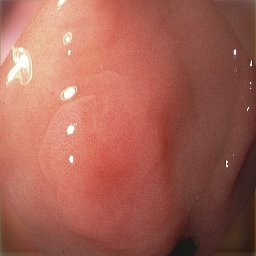
\includegraphics[width=\textwidth]{experiments/figures/blackcorner/polypAE.jpg}
            \caption[Is this in use]%
            {{\small Image from the polyp class at 256x256 px, generated by an autoencoder }}    
            \label{fig:polyp_AE_CORNER1}
        \end{subfigure}
        \qquad
        \begin{subfigure}[b]{0.4\textwidth}  
            \centering 
            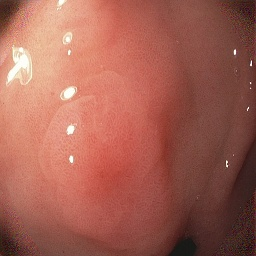
\includegraphics[width=\textwidth]{experiments/figures/blackcorner/polypGAN.jpg}
            \caption[Hate to be this guy]%
            {{\small Image from the polyp class at 256x256 px, generated by a GAN \\.}}    
            \label{fig:polyp_GAN_CORNER1}
        \end{subfigure}
        \qquad\vfill%\vskip\baselineskip
        \begin{subfigure}[b]{0.4\textwidth}   
            \centering 
            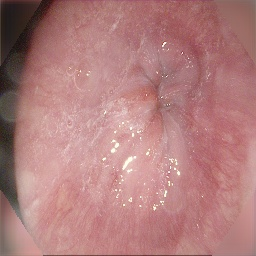
\includegraphics[width=\textwidth]{experiments/figures/blackcorner/zAE.jpg}
            \caption[]%
            {{\small Image from the normal-z-line class at 256x256 px, generated by an autoencoder }}    
            \label{fig:z_AE_CORNER1}
        \end{subfigure}
        \qquad%\hfill%\quad
        \begin{subfigure}[b]{0.4\textwidth}   
            \centering 
            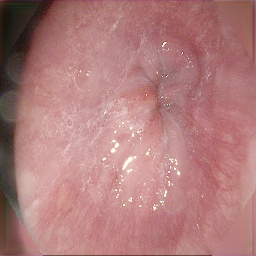
\includegraphics[width=\textwidth]{experiments/figures/blackcorner/zGAN.jpg}
            \caption[]%
            {{\small Image from the normal-z-line class at 256x256 px, generated by a GAN }}    
            \label{fig:z_GAN_CORNER1}
        \end{subfigure}
        \caption[ ]
        {\small Two images from the polyp class and the z-line class. Images on the left were inpained with an Autoencoder, and the images on the right were inpainted with a GAN} 
        \label{fig:AE_GAN_CORNER1}
    \end{figure}
    
        \begin{figure}
        \centering
        \begin{subfigure}[b]{0.4\textwidth}
            \centering
            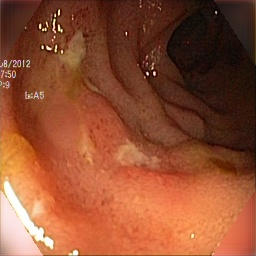
\includegraphics[width=\textwidth]{experiments/figures/blackcorner/ucAE.jpg}
            \caption[Is this in use]%
            {{\small Image from the ulcerative colitis class at 256x256 px, generated by an autoencoder }}    
            \label{fig:polyp_AE_CORNER2}
        \end{subfigure}
        \qquad
        \begin{subfigure}[b]{0.4\textwidth}  
            \centering 
            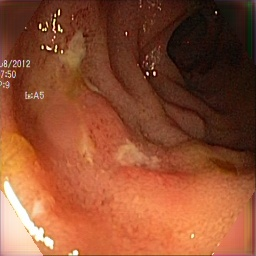
\includegraphics[width=\textwidth]{experiments/figures/blackcorner/ucGAN.jpg}
            \caption[Hate to be this guy]%
            {{\small Image from the ulcerative colitis class at 256x256 px, generated by a GAN}}    
            \label{fig:polyp_GAN_CORNER2}
        \end{subfigure}
        \qquad\vfill%\vskip\baselineskip
        \begin{subfigure}[b]{0.4\textwidth}   
            \centering 
            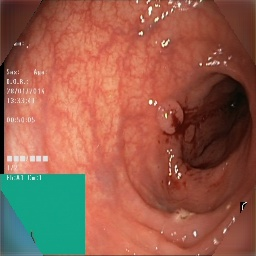
\includegraphics[width=\textwidth]{experiments/figures/blackcorner/polypwithgreenAE.jpg}
            \caption[]%
            {{\small Image from the polyp class at 256x256 px, generated by an autoencoder }}    
            \label{fig:z_AE_CORNER2}
        \end{subfigure}
        \qquad%\hfill%\quad
        \begin{subfigure}[b]{0.4\textwidth}   
            \centering 
            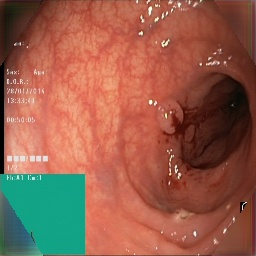
\includegraphics[width=\textwidth]{experiments/figures/blackcorner/polypwithgreenGAN.jpg}
            \caption[]%
            {{\small Image from the polyp class at 256x256 px, generated by a GAN\\. }}    
            \label{fig:z_GAN_CORNER2}
        \end{subfigure}
        \caption[ ]
        {\small Two images from the polyp class and the ulcerative colitis. Here we see results that are not up to a good standard with regards to to light and to green colours.} 
        \label{fig:AE_GAN_CORNER2}
    \end{figure}
    
Here we have presented representative images from both datasets inpainting the four edges around the image. Figure \ref{fig:AE_GAN_CORNER1} show images that, for both dataset are well inpainted, and could pass as real images.
We can discern that, in general, the autoencoder dataset gives a much more blurry image compared to the dataset generated by the GAN.

\ref{fig:AE_GAN_CORNER2} show images that are more problematic. In Figure \ref{fig:polyp_AE_CORNER2} the image generated by the Autoencoder has drawn its colour from the nearby white oversaturated area, and subsequently, it has misdrawn the corner. In Figure \ref{fig:polyp_GAN_CORNER2} we do not have the same problem, as it has drawn information from a larger part of the image, and hence not drawn the oversaturated area.
Both models failed in getting the right colour for the green box when present.

\subsection{Green square}
The next two datasets were generated from the mask in Figure \ref{fig:square_mask}.  The goal of the datasets generated by the Autoencoder and the GAN is to remove the dataset-specific green square. 


        \begin{figure}
        \centering
        \begin{subfigure}[b]{0.4\textwidth}
            \centering
            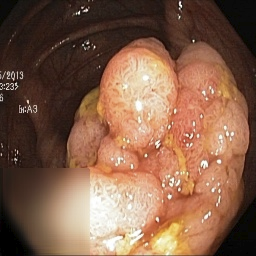
\includegraphics[width=\textwidth]{experiments/figures/greensquare/polypAE.png}
            \caption[Is this in use]%
            {{\small Image from the polyp class at 256x256 px, generated by an autoencoder }}    
            \label{fig:polyp_AE_SQUARE1}
        \end{subfigure}
        \qquad
        \begin{subfigure}[b]{0.4\textwidth}  
            \centering 
            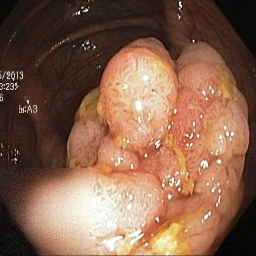
\includegraphics[width=\textwidth]{experiments/figures/greensquare/polypGAN.png}
            \caption[Hate to be this guy]%
            {{\small Image from the polyp class at 256x256 px, generated by a GAN \\.}}    
            \label{fig:polyp_GAN_SQUARE1}
        \end{subfigure}
        \qquad\vfill%\vskip\baselineskip
        \begin{subfigure}[b]{0.4\textwidth}   
            \centering 
            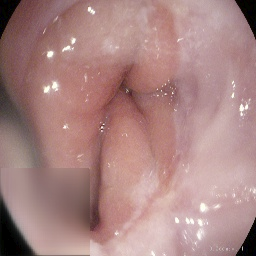
\includegraphics[width=\textwidth]{experiments/figures/greensquare/zAE.png}
            \caption[]%
            {{\small Image from the normal-z-line class at 256x256 px, generated by an autoencoder }}    
            \label{fig:z_AE_SQUARE1}
        \end{subfigure}
        \qquad%\hfill%\quad
        \begin{subfigure}[b]{0.4\textwidth}   
            \centering 
            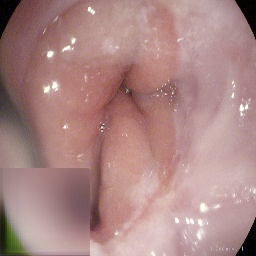
\includegraphics[width=\textwidth]{experiments/figures/greensquare/zGAN.png}
            \caption[]%
            {{\small Image from the normal-z-line class at 256x256 px, generated by a GAN }}    
            \label{fig:z_GAN_SQUARE1}
        \end{subfigure}
        \caption[ ]
        {\small Two images from the polyp class and the normal-z-line class. Here we see results that needed finer detail when inpainting.} 
        \label{fig:AE_GAN_SQUARE1}
    \end{figure}
    
    \begin{figure}
        \centering
        \begin{subfigure}[b]{0.4\textwidth}
            \centering
            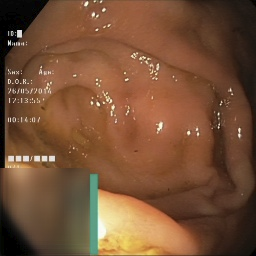
\includegraphics[width=\textwidth]{experiments/figures/greensquare/normalmissAE.png}
            \caption[Is this in use]%
            {{\small Image from the polyp class at 256x256 px, generated by an autoencoder }}    
            \label{fig:polyp_AE_SQUARE2}
        \end{subfigure}
        \qquad
        \begin{subfigure}[b]{0.4\textwidth}  
            \centering 
            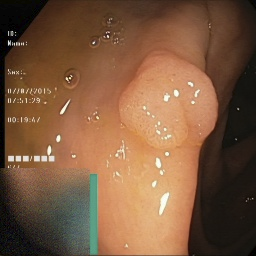
\includegraphics[width=\textwidth]{experiments/figures/greensquare/normalmissGAN.png}
            \caption[Hate to be this guy]%
            {{\small Image from the polyp class at 256x256 px, generated by a GAN \\.}}    
            \label{fig:polyp_GAN_SQUARE2}
        \end{subfigure}
        \qquad\vfill%\vskip\baselineskip
        \begin{subfigure}[b]{0.4\textwidth}   
            \centering 
            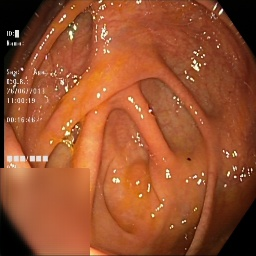
\includegraphics[width=\textwidth]{experiments/figures/greensquare/ncAE.jpg}
            \caption[]%
            {{\small Image from the normal-cecum class at 256x256 px, generated by an autoencoder }}    
            \label{fig:nc_AE_SQUARE2}
        \end{subfigure}
        \qquad%\hfill%\quad
        \begin{subfigure}[b]{0.4\textwidth}   
            \centering 
            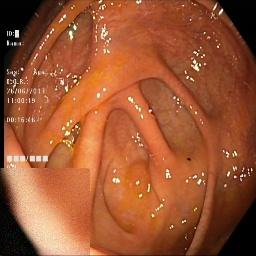
\includegraphics[width=\textwidth]{experiments/figures/greensquare/ncGAN.jpg}
            \caption[]%
            {{\small Image from the normal-cecum class at 256x256 px, generated by a GAN }}    
            \label{fig:nc_GAN_SQUARE2}
        \end{subfigure}
        \caption[ ]
        {\small Two images from the polyp class and the normal-cecum class. Here we have images with a problematic green square, and an image with non-essential details.} 
        \label{fig:AE_GAN_SQUARE2}
    \end{figure}
    
Figure \ref{fig:AE_GAN_SQUARE1} and Figure \ref{fig:AE_GAN_SQUARE2} shows two exaples from the datasets with the green square inpainted.
The images in both figures showcase in detail how the different algorithms inpaints larger areas. \todo{rewrite}

Figure \ref{fig:nc_GAN_SQUARE2} and Figure \ref{fig:z_AE_SQUARE1} shows examples where the GAN has made a better prediction of the complex structures that lie behind the masked area.
We also have an example where the network gets an unconventional input, resulting in discolouration of the target area.         
    \subsection{Combination}
        \begin{figure}
        \centering
        \begin{subfigure}[b]{0.4\textwidth}
            \centering
            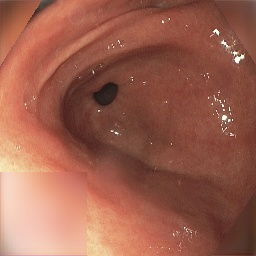
\includegraphics[width=\textwidth]{experiments/figures/both/NPAE.jpg}
            \caption[Is this in use]%
            {{\small Image from the normal-pylorus class at 256x256 px, generated by an autoencoder }}    
            \label{fig:polypAEGREEN}
        \end{subfigure}
        \qquad
        \begin{subfigure}[b]{0.4\textwidth}  
            \centering 
            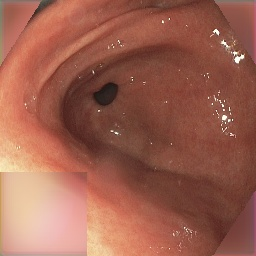
\includegraphics[width=\textwidth]{experiments/figures/both/NPGAN.jpg}
            \caption[Hate to be this guy]%
            {{\small Image from the normal-pylorus class at 256x256 px, generated by a GAN }}    
            \label{fig:polypGAN}
        \end{subfigure}
        \qquad\vfill%\vskip\baselineskip
        \begin{subfigure}[b]{0.4\textwidth}   
            \centering 
            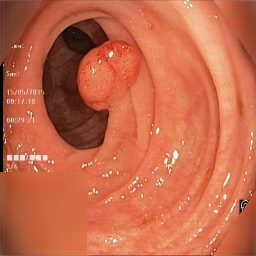
\includegraphics[width=\textwidth]{experiments/figures/both/PAE.jpg}
            \caption[]%
            {{\small Image from the polyp class at 256x256 px, generated by an autoencoder }}    
            \label{fig:zAE}
        \end{subfigure}
        \qquad%\hfill%\quad
        \begin{subfigure}[b]{0.4\textwidth}   
            \centering 
            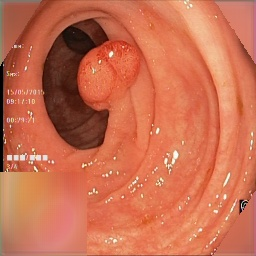
\includegraphics[width=\textwidth]{experiments/figures/both/PGAN.jpg}
            \caption[]%
            {{\small Image from the polyp class at 256x256 px, generated by a GAN \\.}}    
            \label{fig:zGAN}
        \end{subfigure}
        \caption[ ]
        {\small New text here} 
        \label{fig:GC1GREEN}
    \end{figure}
    
    \begin{figure}
        \centering
        \begin{subfigure}[b]{0.4\textwidth}
            \centering
            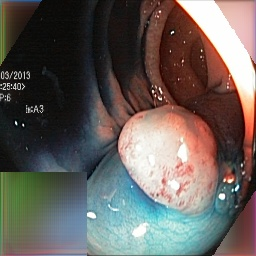
\includegraphics[width=\textwidth]{experiments/figures/both/DLAE.jpg}
            \caption[Is this in use]%
            {{\small Image from the dye lifted polyp class at 256x256 px, generated by an autoencoder }}    
            \label{fig:polypAEGREEN}
        \end{subfigure}
        \qquad
        \begin{subfigure}[b]{0.4\textwidth}  
            \centering 
            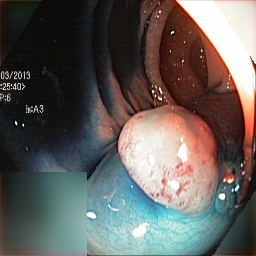
\includegraphics[width=\textwidth]{experiments/figures/both/DLGAN.jpg}
            \caption[Hate to be this guy]%
            {{\small Image from the dye lifted polyp class at 256x256 px, generated by a GAN}}    
            \label{fig:polypGAN}
        \end{subfigure}
        \qquad\vfill%\vskip\baselineskip
        \begin{subfigure}[b]{0.4\textwidth}   
            \centering 
            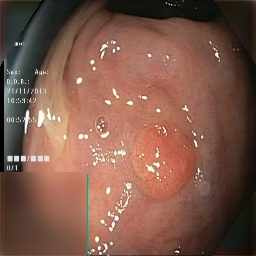
\includegraphics[width=\textwidth]{experiments/figures/both/greenAE.jpg}
            \caption[]%
            {{\small Image from the polyp class at 256x256 px, generated by an autoencoder }}    
            \label{fig:zAE}
        \end{subfigure}
        \qquad%\hfill%\quad
        \begin{subfigure}[b]{0.4\textwidth}   
            \centering 
            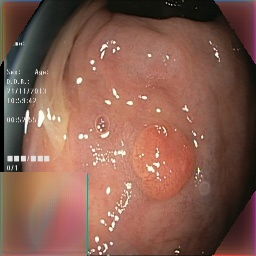
\includegraphics[width=\textwidth]{experiments/figures/both/greenGAN.jpg}
            \caption[]%
            {{\small Image from the polyp class at 256x256 px, generated by a GAN }}    
            \label{fig:zGAN}
        \end{subfigure}
        \caption[ ]
        {\small New text here} 
        \label{fig:GC1GREEN}
    \end{figure}
    

   
\FloatBarrier

\section{Results of the transfer learning experiments}
In the last chapter, we looked at the generation of the new datasets. \textit{we looked at the parameters behind the creation of each of them}, and we discussed downfall and advantages with the autoencoder method versus the GAN method. 

We are now looking at the results when using the newly created datasets when training a classifier for each one of them. 


The model used for the classifier is the same for all the datasets. We use the same learning rate, the same model, and the same parameters for early stopping of the training.  In this section we will first go through the model, then we will look at the results for each of the runs.

\subsection{models}
The clssification models was as follows.
First, we supply info about the model. This information is for instance batch size, type of network, and choice of an optimiser. 

The network chosen is loaded with the imagenet weights. With the model loaded into memory, a global average pooling layer is added, followed by a fully connected layer with the number of nodes equal to the number of classes in the input dataset and a softmax activation step.

With the model loaded we complete it by adding the desired optimiser, and set parameters like batch size, learning rate, validation patience, and image size.

\begin{figure}[h!]
        \centering
        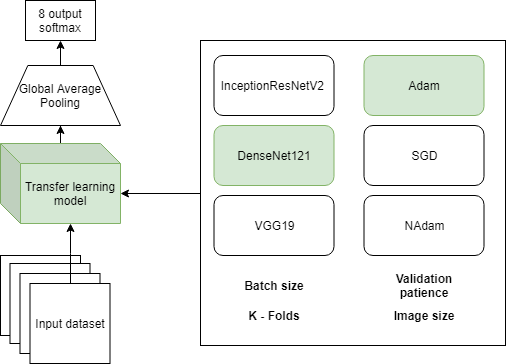
\includegraphics[scale=0.7]{experiments/figures/model.png}
        \caption{ The model we use for classifying with the most important options for the learning process. }
    \label{fig:KTLmodel}
\end{figure}

\todo{here we talk about K-fold}

When we are looking at the models, we use the base case results as a reference point improve upon. This base case is the result of a standard run of classification without any inpainting.

\begin{table}[h]
\caption{Attributes for the training}
\begin{center}
\begin{tabular}{ll}
\toprule
Atribute                                                                              & Value   \\
\midrule
Max Number of epochs                                                                  & 20      \\
\begin{tabular}[c]{@{}l@{}}Patience for \\ validation to improve\end{tabular} & 3       \\
Folds                                                                                 & 6       \\
Image size                                                                            & 256x256 \\
Batch size                                                                            & 6   \\   
\bottomrule
\end{tabular}
\end{center}
\label{tab:I}
\end{table}

\FloatBarrier
\clearpage
\section{Densenet121}

Based on the hyperparameter-optimiser SAGA\todo{ref saga/rune} we have the optimal network to achieve the highest score when both training and evaluating on the Kvasir dataset. 
The Densenet121 model gets its name from the use of fully connected blocks between the convolutional layers. 

Based on the SAGA results, we assume that Densenet121 will give the best results both when evaluating our network on the Kvasir dataset, and when we use the generalised models on the CVC datasets.
The stats for the Densenet training routine is shown in Table \ref{tab:TrainingAttrDN121}.



\begin{table}[h]
\caption{Training attributes for Densenet121 base model }
\begin{center}
\begin{tabular}{ll}
\toprule
Atribute                & Value   \\
\midrule
Max Number of epochs    & 20      \\
Patience for validation & 3       \\
Folds                   & 6       \\
Image size              & 256x256 \\
Batch size              & 24      \\   
\bottomrule
\end{tabular}
\end{center}
\label{tab:TrainingAttrDN121}
\end{table}

The parameters used are to get the optimal amount of training without overfitting to the data. We have chosen training patience of three. This patience is a compromise between a higher value, more likely to overfit, and a lower value, more likely to stop too early to learn all the meaningful representations. 


\clearpage
\subsection{Densenet121 base model}

We present the results with Densenet121 in table \ref{fig:results_IRV2_base}.
This Table shows the base case result with the Densenet121 model. 

\begin{figure}[h]
\caption{Densenet121 Base results}
\myfontsize
%\advance\leftskip-1.5cm
\caption*{\footnotesize \textmd{ \textbf{A}:{dyed-lifted-polyps} , \textbf{B}:{dyed-resection-margins} , \textbf{C}:{esophagitis} , \textbf{D}:{normal-cecum} , \textbf{E}:{normal-pylorus} , \textbf{F}:{normal-z-line} , \textbf{G}:{polyps} , \textbf{H}:{ulcerative-colitis} , \textbf{I}:{non-polyp}}}

\begin{subfigure}[b]{0.25\textwidth}
     
\[
\begin{blockarray}{ccc}
& I & G  \\
\begin{block}{c[cc]}
        I&1310 &  37\\
        G& 618 &  319\\
\end{block}
\end{blockarray}
 \]         

\caption{Baseline Confusion matrix for the CVC 356 dataset}
\label{mat:cvc356_CM_DN121_base}
\end{subfigure}
\begin{subfigure}[b]{0.49\textwidth}  
\scriptsize     
\[
\begin{blockarray}{ccccccccc}
& A & B & C & D & E & F & G & H \\
\begin{block}{c[cccccccc]}
A&150 & 6 & 0 & 0 & 0 & 0 & 1 & 0\\
B& 14 & 160 & 0 & 0 & 0 & 0 & 0 & 0\\
C&  0 & 0 & 130 & 0 & 1 & 19 & 0 & 0\\
D&  0 & 0 & 0 & 162 & 0 & 0 & 1 & 3\\
E&  0 & 0 & 0 & 0 & 164 & 0 & 0 & 0\\
F&  0 & 0 & 36 & 0 & 0 & 147 & 1 & 0\\
G&  1 & 0 & 0 & 3 & 1 & 0 & 161 & 2\\
H&  1 & 0 & 0 & 1 & 0 & 0 & 2 & 161\\
\end{block}
\end{blockarray}
 \]        
        
        
\caption{Baseline Confusion matrix for the Kvasir dataset}
\label{mat:kvasir_CM_DN121_base}
\end{subfigure}
\begin{subfigure}[b]{0.25\textwidth}
        \[
\begin{blockarray}{ccc}
& I & G  \\
\begin{block}{c[cc]}
 		I&1311 & 3553\\
        G&618  & 6472\\
\end{block}
\end{blockarray}
\]   
\caption{Baseline Confusion matrix for the CVC 12k dataset}
\label{mat:cvc12k_CM_DN121_base}
\end{subfigure}
\caption{Confusion matrices for the three datasets}
\label{mat:CM_DN121_base}
\begin{subfigure}[b]{0.25\textwidth}
\begin{tabular}{ll}      
        \toprule
        \multicolumn{2}{c}{CVC 356 dataset}        \\
        \midrule
        MCC 		& 0.4244 \\
        F1  		& 0.6467 \\
        Precicion  	& 0.7878 \\
        Recall     	& 0.6565 \\
        Accuracy	& 0.7132 \\
        \bottomrule
        \end{tabular}
\caption{The CVC 356 dataset Metrics}
\label{tab:cvc356_metrics_DN121_base}
\end{subfigure}%
\begin{subfigure}[b]{0.49\textwidth}
    	\centering
        \begin{tabular}{ll}
        \toprule
        \multicolumn{2}{c}{Kvasir dataset}        \\
        \midrule
        MCC 		& 0.9202 \\
        F1  		& 0.9299 \\
        Precicion  	& 0.93 \\
        Recall     	& 0.9313  \\
        Accuracy	& 0.93 \\
        
        \bottomrule
\end{tabular}
\caption{The Kvasir dataset\\ Metrics}
\label{tab:kvasir_metrics_DN121_base}
\end{subfigure}%
\begin{subfigure}[b]{0.25\textwidth}
        \begin{tabular}{ll}
        \toprule
        \multicolumn{2}{c}{CVC 12k dataset}        \\
        \midrule
        MCC 		& 0.2435  \\
        F1  		& 0.5711 \\
        Precicion  	& 0.6626 \\
        Recall     	& 0.5912 \\
        Accuracy	& 0.6511 \\
        \bottomrule
        \end{tabular}
\caption{The CVC 12k dataset Metrics}
\label{tab:cvc12k_metrics_DN121_base}
\end{subfigure}
\caption{The baseline confusion matrixes}
\label{fig:results_DN121_base}
%\advance\rightskip-1.5cm
\end{figure}


\FloatBarrier
\noindent


Matrix \ref{mat:CM_DN121_base} shows the evaluation of the test set on each of the three datasets used. 
On the Kvasir dataset, we used five folds for training and validation, and the last sixth fold for the testing. That left us with 1342 images divided evenly between the classes. 

\paragraph{CVC 356}
The CVC 356 base case MCC lies at 0.42 with an accuracy of 71\%. 
From the Confusion matrix we can discern that most polyps were classified correctly, except for the case that 37 of the images did not classify as a polyp when it was. Moreover, we also had 618 cases of non-polyps classified as polyps.

\paragraph{The Kvasir}
In this Confusion matrix, we see that most of the samples lie throughout the diagonal, which, as we recall, is the correct classification. 
The Kvasir base case MCC lies at 0.92 which coincides with an near perfect accuracy given the complexity of the dataset.

\paragraph{CVC 12k}
The CVC 356 base case MCC lies at 0.24 with an accuracy of 65\%. 
From the Confusion matrix we can discern that most polyps were classified correctly, though a third of the polyps were misclassified.






\subsection{Corners inpainted result}
Based on Hypothesis \ref{hyp:b} we would expect the act of inpainting the corner in the images to give Kvasir a higher score complared to the baseline. In addition, we could see improvement in both CVC 356 and CVC 12k.
We present the GAN followed by the Autoencoder and evaluate them together.


\begin{figure}
\caption{Densenet121 Inpainted corners with the GAN results}
\myfontsize
%\advance\leftskip-1.5cm
\caption*{\footnotesize \textmd{ \textbf{A}:{dyed-lifted-polyps} , \textbf{B}:{dyed-resection-margins} , \textbf{C}:{esophagitis} , \textbf{D}:{normal-cecum} , \textbf{E}:{normal-pylorus} , \textbf{F}:{normal-z-line} , \textbf{G}:{polyps} , \textbf{H}:{ulcerative-colitis} , \textbf{I}:{non-polyp}}}

\begin{subfigure}[b]{0.25\textwidth}
     
\[
\begin{blockarray}{ccc}
& I & G  \\
\begin{block}{c[cc]}
        I&1647 &  179\\
        G& 281 &  177\\
\end{block}
\end{blockarray}
 \]         

\caption{GAN corners Confusion matrix for the CVC 356 dataset}
\label{mat:cvc356_CM_DN121_GAN_CORNER}
\end{subfigure}
\begin{subfigure}[b]{0.49\textwidth}  
\scriptsize     
\[
\begin{blockarray}{ccccccccc}
& A & B & C & D & E & F & G & H \\
\begin{block}{c[cccccccc]}
A&157 & 12 & 0 & 0 & 0 & 0 & 0 & 0\\
B&  8 & 154 & 0 & 0 & 0 & 0 & 0 & 0\\
C&  0 & 0 & 116 & 0 & 0 & 11 & 0 & 0\\
D&  0 & 0 & 0 & 162 & 0 & 0 & 3 & 5\\
E&  0 & 0 & 1 & 0 & 166 & 0 & 3 & 0\\
F&  0 & 0 & 49 & 0 & 0 & 155 & 1 & 0\\
G&  1 & 0 & 0 & 2 & 0 & 0 & 158 & 2\\
H&  0 & 0 & 0 & 2 & 0 & 0 & 1 & 159\\
\end{block}
\end{blockarray}
 \]        
        
        
\caption{GAN corners Confusion matrix for the Kvasir dataset}
\label{mat:kvasir_CM_DN121_GAN_CORNER}
\end{subfigure}
\begin{subfigure}[b]{0.25\textwidth}
        \[
\begin{blockarray}{ccc}
& I & G  \\
\begin{block}{c[cc]}
 		I&1648 & 4699\\
        G&281  & 5326\\
\end{block}
\end{blockarray}
\]   
\caption{GAN corners Confusion matrix for the CVC 12k dataset}
\label{mat:cvc12k_CM_DN121_GAN_CORNER}
\end{subfigure}
\caption{Confusion matrices for the three datasets}
\label{mat:CM_DN121_GAN_CORNER}
\begin{subfigure}[b]{0.25\textwidth}
\begin{tabular}{ll}      
        \toprule
        \multicolumn{2}{c}{CVC 356 dataset}        \\
        \midrule
        MCC 		& 0.3184 \\
        F1  		& 0.6562 \\
        Precicion  	& 0.6757 \\
        Recall     	& 0.6442 \\
        Accuracy	& 0.7986 \\
        \bottomrule
        \end{tabular}
\caption{The CVC 356 dataset Metrics}
\label{tab:cvc356_metrics_DN121_GAN_CORNER}
\end{subfigure}%
\begin{subfigure}[b]{0.49\textwidth}
    	\centering
        \begin{tabular}{ll}
        \toprule
        \multicolumn{2}{c}{Kvasir dataset}        \\
        \midrule
        MCC 		& 0.914 \\
        F1  		& 0.9233 \\
        Precicion  	& 0.9239 \\
        Recall     	& 0.9287 \\
        Accuracy	& 0.9239 \\
        \bottomrule
\end{tabular}
\caption{The Kvasir dataset\\ Metrics}
\label{tab:kvasir_metrics_DN121_GAN_CORNER}
\end{subfigure}%
\begin{subfigure}[b]{0.25\textwidth}
        \begin{tabular}{ll}
        \toprule
        \multicolumn{2}{c}{CVC 12k dataset}        \\
        \midrule
        MCC 		& 0.2842 \\
        F1  		& 0.5398 \\
        Precicion  	& 0.6928 \\
        Recall     	& 0.6048 \\
        Accuracy	& 0.5834 \\
        \bottomrule
        \end{tabular}
\caption{The CVC 12k dataset Metrics}
\label{tab:cvc12k_metrics_DN121_GAN_CORNER}
\end{subfigure}
\caption{The inpainted corner with GAN confusion matrixes}
\label{fig:results_DN121_GAN_CORNER}
%\advance\rightskip-1.5cm
\end{figure}
\FloatBarrier

%Our results from figure \ref{fig:results_IRV2_GAN_CORNER} shows a clear advantage when evaluating the results on the CVC 12K dataset while keeping the result the same on the CVC 256 and Kvasir dataset. %We can not draw any clear conclutions.



\begin{figure}
\caption{Densenet121 Inpainted corners with the AE results}
\myfontsize
%\advance\leftskip-1.5cm
\caption*{\footnotesize \textmd{ \textbf{A}:{dyed-lifted-polyps} , \textbf{B}:{dyed-resection-margins} , \textbf{C}:{esophagitis} , \textbf{D}:{normal-cecum} , \textbf{E}:{normal-pylorus} , \textbf{F}:{normal-z-line} , \textbf{G}:{polyps} , \textbf{H}:{ulcerative-colitis} , \textbf{I}:{non-polyp}}}

\begin{subfigure}[b]{0.25\textwidth}
     
\[
\begin{blockarray}{ccc}
& I & G  \\
\begin{block}{c[cc]}
        I&1746 & 106\\
        G&  182 & 250\\
\end{block}
\end{blockarray}
 \]         

\caption{AE corners Confusion matrix for the CVC 356 dataset}
\label{mat:cvc356_CM_DN121_AE_CORNER}
\end{subfigure}
\begin{subfigure}[b]{0.49\textwidth}  
\scriptsize     
\[
\begin{blockarray}{ccccccccc}
& A & B & C & D & E & F & G & H \\
\begin{block}{c[cccccccc]}
A&150 & 9 & 0 & 0 & 0 & 0 & 1 & 0\\
B& 12 & 157 & 0 & 0 & 0 & 0 & 0 & 0\\
C&  0 & 0 & 141 & 0 & 0 & 21 & 0 & 0\\
D&  1 & 0 & 0 & 160 & 0 & 0 & 4 & 2\\
E&  0 & 0 & 0 & 0 & 166 & 0 & 1 & 0\\
F&  0 & 0 & 25 & 0 & 0 & 145 & 0 & 0\\
G&  3 & 0 & 0 & 3 & 0 & 0 & 157 & 2\\
H&  0 & 0 & 0 & 3 & 0 & 0 & 3 & 162\\
\end{block}
\end{blockarray}
 \]        
        
        
\caption{AE corners Confusion matrix for the Kvasir dataset}
\label{mat:kvasir_CM_DN121_AE_CORNER}
\end{subfigure}
\begin{subfigure}[b]{0.25\textwidth}
        \[
\begin{blockarray}{ccc}
& I & G  \\
\begin{block}{c[cc]}
 		I&1747 & 5227\\
        G&182  & 4798\\
\end{block}
\end{blockarray}
\]   
\caption{AE corners Confusion matrix for the CVC 12k dataset}
\label{mat:cvc12k_CM_DN121_AE_CORNER}
\end{subfigure}
\caption{Confusion matrices for the three datasets}
\label{mat:CM_DN121_AE_CORNER}
\begin{subfigure}[b]{0.25\textwidth}
\begin{tabular}{ll}      
        \toprule
        \multicolumn{2}{c}{CVC 356 dataset}        \\
        \midrule
        MCC 		& 0.563 \\
        F1  		& 0.7792 \\
        Precicion  	& 0.8039 \\
        Recall     	& 0.7607 \\
        Accuracy	& 0.8739 \\
        \bottomrule
        \end{tabular}
\caption{The CVC 356 dataset Metrics}
\label{tab:cvc356_metrics_DN121_AE_CORNER}
\end{subfigure}%
\begin{subfigure}[b]{0.49\textwidth}
    	\centering
        \begin{tabular}{ll}
        \toprule
        \multicolumn{2}{c}{Kvasir dataset}        \\
        \midrule
        MCC 		& 0.9226 \\
        F1  		& 0.9321 \\
        Precicion  	& 0.9322 \\
        Recall     	& 0.9322 \\
        Accuracy	& 0.9322 \\
        \bottomrule
\end{tabular}
\caption{The Kvasir dataset\\ Metrics}
\label{tab:kvasir_metrics_DN121_AE_CORNER}
\end{subfigure}%
\begin{subfigure}[b]{0.25\textwidth}
        \begin{tabular}{ll}
        \toprule
        \multicolumn{2}{c}{CVC 12k dataset}        \\
        \midrule
        MCC 		& 0.2867 \\
        F1  		& 0.516  \\
        Precicion  	& 0.6921 \\
        Recall     	& 0.607 \\
        Accuracy	& 0.5475 \\
        \bottomrule
        \end{tabular}
\caption{The CVC 12k dataset Metrics}
\label{tab:cvc12k_metrics_DN121_AE_CORNER}
\end{subfigure}
\caption{The inpainted corner with AE confusion matrixes}
\label{fig:results_DN121_AE_CORNER}
%\advance\rightskip-1.5cm
\end{figure}
\FloatBarrier

%
Figure \ref{fig:results_DN121_AE_CORNER} and \ref{fig:results_DN121_GAN_CORNER}  shows the evaluation of the test set on each of the three datasets used both for the Autoencoder and GAN. 

\paragraph{CVC 356}
We got the highest MCC from the Autoencoder with a score of 0.56 compared to a score of 0.31 from the GAN.
In general the Autoencoder has a higher score overall compared to the GAN, where the Autoencoder reaches a higher score than the base case, and the GAN does not.


\paragraph{The Kvasir}
When evaluating our results on the Kvasir dataset we see similar scores for both the GAN and Autoencoder with 0.91 and 0.92 respectively. Here the Autoencoder reaches a higher score than the base case, though the margin is too small to significant.

\paragraph{CVC 12k}
The MCC scores for the GAN and Autoencoder both reaches a higher value than the base case. When inpainting the corners we see an increase in MCC value of 0.04 for both methods, giving some indication that removing areas with sparse information might give a higher classification score on other datasets with the same sparse areas.





































\subsection{Square inpainted result}


We can recall from Hypothesis \ref{hyp:a} that removing dataset specific artefacts we will achieve a higher classification score when evaluation our models on previously unseen datasets.
We expect the Kvasir dataset not show any improvements, though both the CVC 356 and the CVC 12k dataset we expect to improve compared to the base case. 
We present the GAN followed by the Autoencoder and evaluate them together.


\begin{figure}
\caption{Densenet121 Inpainted green square with the GAN results}
\myfontsize
%\advance\leftskip-1.5cm
\caption*{\footnotesize \textmd{ \textbf{A}:{dyed-lifted-polyps} , \textbf{B}:{dyed-resection-margins} , \textbf{C}:{esophagitis} , \textbf{D}:{normal-cecum} , \textbf{E}:{normal-pylorus} , \textbf{F}:{normal-z-line} , \textbf{G}:{polyps} , \textbf{H}:{ulcerative-colitis} , \textbf{I}:{non-polyp}}}

\begin{subfigure}[b]{0.25\textwidth}
     
\[
\begin{blockarray}{ccc}
& I & G  \\
\begin{block}{c[cc]}
        I&1848 &  92\\
        G& 80 &  264\\
\end{block}
\end{blockarray}
 \]         

\caption{GAN green square Confusion matrix for the CVC 356 dataset}
\label{mat:cvc356_CM_DN121_GAN_SQUARE}
\end{subfigure}
\begin{subfigure}[b]{0.49\textwidth}  
\scriptsize     
\[
\begin{blockarray}{ccccccccc}
& A & B & C & D & E & F & G & H \\
\begin{block}{c[cccccccc]}
A&157 & 13 & 0 & 0 & 0 & 0 & 0 & 0\\
B&  7 & 153 & 0 & 0 & 0 & 0 & 0 & 0\\
C&  0 & 0 & 146 & 0 & 1 & 37 & 0 & 0\\
D&  0 & 0 & 0 & 161 & 0 & 0 & 8 & 4\\
E&  0 & 0 & 1 & 0 & 165 & 1 & 1 & 0\\
F&  0 & 0 & 19 & 0 & 0 & 128 & 0 & 0\\
G&  2 & 0 & 0 & 3 & 0 & 0 & 153 & 0\\
H&  0 & 0 & 0 & 2 & 0 & 0 & 4 & 162\\
\end{block}
\end{blockarray}
 \]        
        
        
\caption{GAN green square Confusion matrix for the Kvasir dataset}
\label{mat:kvasir_CM_DN121_GAN_SQUARE}
\end{subfigure}
\begin{subfigure}[b]{0.25\textwidth}
        \[
\begin{blockarray}{ccc}
& I & G  \\
\begin{block}{c[cc]}
 		I&1849 & 6850\\
        G&  80 & 3175\\
\end{block}
\end{blockarray}
\]   
\caption{GAN green square Confusion matrix for the CVC 12k dataset}
\label{mat:cvc12k_CM_DN121_GAN_SQUARE}
\end{subfigure}
\caption{Confusion matrices for the three datasets}
\label{mat:CM_DN121_GAN_SQUARE}
\begin{subfigure}[b]{0.25\textwidth}
\begin{tabular}{ll}      
        \toprule
        \multicolumn{2}{c}{CVC 356 dataset}        \\
        \midrule
        MCC 		& 0.71 \\
        F1  		& 0.8549 \\
        Precicion  	& 0.85 \\
        Recall     	& 0.86 \\
        Accuracy	& 0.9247  \\         
        \bottomrule
        \end{tabular}
\caption{The CVC 356 dataset Metrics}
\label{tab:cvc356_metrics_DN121_GAN_SQUARE}
\end{subfigure}%
\begin{subfigure}[b]{0.49\textwidth}
    	\centering
        \begin{tabular}{ll}
        \toprule
        \multicolumn{2}{c}{Kvasir dataset}        \\
        \midrule
        MCC 		& 0.9116 \\
        F1  		& 0.9222  \\
        Precicion  	& 0.9224 \\
        Recall     	& 0.9237 \\
        Accuracy	& 0.9224 \\
        \bottomrule
\end{tabular}
\caption{The Kvasir dataset\\ Metrics}
\label{tab:kvasir_metrics_DN121_GAN_SQUARE}
\end{subfigure}%
\begin{subfigure}[b]{0.25\textwidth}
        \begin{tabular}{ll}
        \toprule
        \multicolumn{2}{c}{CVC 12k dataset}        \\
        \midrule
        MCC 		& 0.2275 \\
        F1  		& 0.4131 \\
        Precicion  	& 0.6376 \\
        Recall     	& 0.594 \\
        Accuracy	& 0.4203 \\
        \bottomrule
        \end{tabular}
\caption{The CVC 12k dataset Metrics}
\label{tab:cvc12k_metrics_DN121_GAN_SQUARE}
\end{subfigure}
\caption{The inpainted green square with GAN confusion matrixes}
\label{fig:results_DN121_GAN_SQUARE}
%\advance\rightskip-1.5cm
\end{figure}
\FloatBarrier



\begin{figure}
\caption{Densenet121 Inpainted green square with the AE results}
\myfontsize
%\advance\leftskip-1.5cm
\caption*{\footnotesize \textmd{ \textbf{A}:{dyed-lifted-polyps} , \textbf{B}:{dyed-resection-margins} , \textbf{C}:{esophagitis} , \textbf{D}:{normal-cecum} , \textbf{E}:{normal-pylorus} , \textbf{F}:{normal-z-line} , \textbf{G}:{polyps} , \textbf{H}:{ulcerative-colitis} , \textbf{I}:{non-polyp}}}

\begin{subfigure}[b]{0.25\textwidth}
     
\[
\begin{blockarray}{ccc}
& I & G  \\
\begin{block}{c[cc]}
        I&1746 & 106\\
        G&  182 & 250\\
\end{block}
\end{blockarray}
 \]         

\caption{AE green square Confusion matrix for the CVC 356 dataset}
\label{mat:cvc356_CM_DN121_AE_SQUARE}
\end{subfigure}
\begin{subfigure}[b]{0.49\textwidth}  
\scriptsize     
\[
\begin{blockarray}{ccccccccc}
& A & B & C & D & E & F & G & H \\
\begin{block}{c[cccccccc]}
A&150 & 9 & 0 & 0 & 0 & 0 & 1 & 0\\
B& 12 & 157 & 0 & 0 & 0 & 0 & 0 & 0\\
C&  0 & 0 & 141 & 0 & 0 & 21 & 0 & 0\\
D&  1 & 0 & 0 & 160 & 0 & 0 & 4 & 2\\
E&  0 & 0 & 0 & 0 & 166 & 0 & 1 & 0\\
F&  0 & 0 & 25 & 0 & 0 & 145 & 0 & 0\\
G&  3 & 0 & 0 & 3 & 0 & 0 & 157 & 2\\
H&  0 & 0 & 0 & 3 & 0 & 0 & 3 & 162\\
\end{block}
\end{blockarray}
 \]        
        
        
\caption{AE green square Confusion\\ matrix for the Kvasir dataset}
\label{mat:kvasir_CM_DN121_AE_SQUARE}
\end{subfigure}
\begin{subfigure}[b]{0.25\textwidth}
        \[
\begin{blockarray}{ccc}
& I & G  \\
\begin{block}{c[cc]}
 		I&1747 & 5227\\
        G&182  & 4798\\
\end{block}
\end{blockarray}
\]   
\caption{AE green square Confusion matrix for the CVC 12k dataset}
\label{mat:cvc12k_CM_DN121_AE_SQUARE}
\end{subfigure}
\caption{Confusion matrices for the three datasets}
\label{mat:CM_DN121_AE_SQUARE}
\begin{subfigure}[b]{0.25\textwidth}
\begin{tabular}{ll}      
        \toprule
        \multicolumn{2}{c}{CVC 356 dataset}        \\
        \midrule
        MCC 		& 0.6072 \\
        F1  		& 0.8017 \\
        Precicion  	& 0.8248 \\
        Recall      & 0.7837 \\
        Accuracy	& 0.8879 \\
        \bottomrule
            
        \end{tabular}
\caption{The CVC 356 dataset Metrics}
\label{tab:cvc356_metrics_DN121_AE_SQUARE}
\end{subfigure}%
\begin{subfigure}[b]{0.49\textwidth}
    	\centering
        \begin{tabular}{ll}
        \toprule
        \multicolumn{2}{c}{Kvasir dataset}        \\
        \midrule
        MCC 		& 0.9158 \\
        F1  		& 0.9262  \\
        Precicion  	& 0.9262 \\
        Recall     	& 0.9271  \\
        Accuracy	& 0.9262 \\
        \bottomrule
\end{tabular}
\caption{The Kvasir dataset\\ Metrics}
\label{tab:kvasir_metrics_DN121_AE_SQUARE}
\end{subfigure}%
\begin{subfigure}[b]{0.25\textwidth}
        \begin{tabular}{ll}
        \toprule
        \multicolumn{2}{c}{CVC 12k dataset}        \\
        \midrule
        MCC 		& 0.2029 \\
        F1  		& 0.4185  \\
        Precicion  	& 0.6257 \\
        Recall     	& 0.5819 \\
        Accuracy	& 0.4287 \\
        \bottomrule
        \end{tabular}
\caption{The CVC 12k dataset Metrics}
\label{tab:cvc12k_metrics_DN121_AE_SQUARE}
\end{subfigure}
\caption{The inpainted green square with AE confusion matrixes}
\label{fig:results_DN121_AE_SQUARE}
%\advance\rightskip-1.5cm
\end{figure}
\FloatBarrier

%
Figure \ref{fig:results_DN121_GAN_SQUARE} and \ref{fig:results_DN121_AE_SQUARE} shows the evaluation of the test set on each of the three datasets used both for the GAN and Autoencoder. 

\paragraph{CVC 356}
As this is a dataset unseen by the classifier during training, we would expect, given that Hypothesis \ref{hyp:a} is True, that the classification score would be higher than the base case.
Here we have \textit{significantly} higher score with both the GAN and Autoencoder. 
The GAN reached a MCC score of 0.71 compared to the base case of 42. The Autoencoder also beat the base case with a large margin, given the MCC score of 0.60.

This highly suggest that our hypothesis about removing dataset-specific artefacts to improve accuracy is indeed correct. 

\paragraph{The Kvasir}
As with the previous tests we see little change in the scores when evaluation on the Kvasir dataset.
Here both the GAN and the Autoencoder got a lower score compared to the base, though only with a small margin.


\paragraph{CVC 12k}
As with the CVC 356 dataset the CVC 12k dataset is unseen by the classifier during training. 
Here, both the GAN and Autoencoder reaches a lower MCC value when evaluation on the dataset. 
\todo{This disproves hyp:a}
















































\subsection{Both inpainted result}

In addition to test the two hypothesises separately we, as we recall, want to test both types of inpainting at the same time.
When testing both inpainting types we can not draw any predictions reliably, given that we do not know if the two methods interfere with each other. 

We present the GAN inpainting of both the areas followed by the same inpainting with the Autoencoder.


\begin{figure}
\caption{Densenet121 Inpainted both areas with the GAN results}
\myfontsize
%\advance\leftskip-1.5cm
\caption*{\footnotesize \textmd{ \textbf{A}:{dyed-lifted-polyps} , \textbf{B}:{dyed-resection-margins} , \textbf{C}:{esophagitis} , \textbf{D}:{normal-cecum} , \textbf{E}:{normal-pylorus} , \textbf{F}:{normal-z-line} , \textbf{G}:{polyps} , \textbf{H}:{ulcerative-colitis} , \textbf{I}:{non-polyp}}}

\begin{subfigure}[b]{0.25\textwidth}
     
\[
\begin{blockarray}{ccc}
& I & G  \\
\begin{block}{c[cc]}
        I&1916 &  129\\
        G& 12 &  227\\
\end{block}
\end{blockarray}
 \]         

\caption{GAN both areas Confusion matrix for the CVC 356 dataset}
\label{mat:cvc356_CM_DN121_GAN_BOTH}
\end{subfigure}
\begin{subfigure}[b]{0.49\textwidth}  
\scriptsize     
\[
\begin{blockarray}{ccccccccc}
& A & B & C & D & E & F & G & H \\
\begin{block}{c[cccccccc]}
A&159 & 7 & 0 & 0 & 0 & 0 & 2 & 1\\
B&  7 & 158 & 0 & 0 & 0 & 0 & 0 & 0\\
C&  0 & 0 & 118 & 0 & 0 & 8 & 0 & 0\\
D&  0 & 0 & 0 & 161 & 0 & 0 & 3 & 4\\
E&  0 & 0 & 1 & 0 & 164 & 0 & 3 & 0\\
F&  0 & 0 & 47 & 0 & 0 & 158 & 1 & 0\\
G&  0 & 0 & 0 & 0 & 1 & 0 & 154 & 0\\
H&  0 & 1 & 0 & 5 & 1 & 0 & 3 & 161\\
\end{block}
\end{blockarray}
 \]        
        
        
\caption{GAN both areas Confusion matrix for the Kvasir dataset}
\label{mat:kvasir_CM_DN121_GAN_BOTH}
\end{subfigure}
\begin{subfigure}[b]{0.25\textwidth}
        \[
\begin{blockarray}{ccc}
& I & G  \\
\begin{block}{c[cc]}
 		I&1917 & 7851\\
        G&  12 & 2174\\
\end{block}
\end{blockarray}
\]   
\caption{GAN both areas Confusion matrix for the CVC 12k dataset}
\label{mat:cvc12k_CM_DN121_GAN_BOTH}
\end{subfigure}
\caption{Confusion matrices for the three datasets}
\label{mat:CM_DN121_GAN_BOTH}
\begin{subfigure}[b]{0.25\textwidth}
\begin{tabular}{ll}      
        \toprule
        \multicolumn{2}{c}{CVC 356 dataset}        \\
        \midrule
        MCC 		& 0.7483 \\
        F1  		& 0.8638 \\
        Precicion  	& 0.8157 \\
        Recall      & 0.9434 \\
        Accuracy	& 0.9383  \\         
        \bottomrule
        \end{tabular}
\caption{The CVC 356 dataset Metrics}
\label{tab:cvc356_metrics_DN121_GAN_BOTH}
\end{subfigure}%
\begin{subfigure}[b]{0.49\textwidth}
    	\centering
        \begin{tabular}{ll}
        \toprule
        \multicolumn{2}{c}{Kvasir dataset}        \\
        \midrule
        MCC 		& 0.9192 \\
        F1  		& 0.9278  \\
        Precicion  	& 0.9285 \\
        Recall     	& 0.9339 \\
        Accuracy	& 0.9285 \\
        \bottomrule
\end{tabular}
\caption{The Kvasir dataset\\ Metrics}
\label{tab:kvasir_metrics_DN121_GAN_BOTH}
\end{subfigure}%
\begin{subfigure}[b]{0.25\textwidth}
        \begin{tabular}{ll}
        \toprule
        \multicolumn{2}{c}{CVC 12k dataset}        \\
        \midrule
        MCC 		& 0.2005 \\
        F1  		& 0.3419 \\
        Precicion  	& 0.6053 \\
        Recall     	& 0.5954 \\
        Accuracy	& 0.3422 \\
        \bottomrule
        \end{tabular}
\caption{The CVC 12k dataset Metrics}
\label{tab:cvc12k_metrics_DN121_GAN_BOTH}
\end{subfigure}
\caption{The inpainted both areas with GAN confusion matrixes}
\label{fig:results_DN121_GAN_BOTH}
%\advance\rightskip-1.5cm
\end{figure}
\FloatBarrier



\begin{figure}
\caption{Densenet121 Inpainted both areas with the AE results}
\myfontsize
%\advance\leftskip-1.5cm
\caption*{\footnotesize \textmd{ \textbf{A}:{dyed-lifted-polyps} , \textbf{B}:{dyed-resection-margins} , \textbf{C}:{esophagitis} , \textbf{D}:{normal-cecum} , \textbf{E}:{normal-pylorus} , \textbf{F}:{normal-z-line} , \textbf{G}:{polyps} , \textbf{H}:{ulcerative-colitis} , \textbf{I}:{non-polyp}}}

\begin{subfigure}[b]{0.25\textwidth}
     
\[
\begin{blockarray}{ccc}
& I & G  \\
\begin{block}{c[cc]}
        I&1889 & 238\\
        G&  39 & 118\\
\end{block}
\end{blockarray}
 \]         

\caption{AE both areas Confusion matrix for the CVC 356 dataset}
\label{mat:cvc356_CM_DN121_AE_BOTH}
\end{subfigure}
\begin{subfigure}[b]{0.49\textwidth}  
\scriptsize     
\[
\begin{blockarray}{ccccccccc}
& A & B & C & D & E & F & G & H \\
\begin{block}{c[cccccccc]}
A&149 & 11 & 0 & 0 & 0 & 0 & 1 & 0\\
B& 11 & 155 & 0 & 0 & 0 & 0 & 0 & 0\\
C&  0 & 0 & 143 & 0 & 0 & 25 & 1 & 0\\
D&  0 & 0 & 0 & 156 & 0 & 0 & 0 & 2\\
E&  0 & 0 & 0 & 0 & 166 & 1 & 2 & 1\\
F&  0 & 0 & 23 & 0 & 0 & 140 & 0 & 0\\
G&  4 & 0 & 0 & 5 & 0 & 0 & 154 & 3\\
H&  2 & 0 & 0 & 5 & 0 & 0 & 8 & 160\\
\end{block}
\end{blockarray}
 \]        
        
        
\caption{AE both areas Confusion\\ matrix for the Kvasir dataset}
\label{mat:kvasir_CM_DN121_AE_BOTH}
\end{subfigure}
\begin{subfigure}[b]{0.25\textwidth}
        \[
\begin{blockarray}{ccc}
& I & G  \\
\begin{block}{c[cc]}
 		I&1890 & 7452\\
        G&39  & 2573\\
\end{block}
\end{blockarray}
\]   
\caption{AE both areas Confusion matrix for the CVC 12k dataset}
\label{mat:cvc12k_CM_DN121_AE_BOTH}
\end{subfigure}
\caption{Confusion matrices for the three datasets}
\label{mat:CM_DN121_AE_SQUARE}
\begin{subfigure}[b]{0.25\textwidth}
\begin{tabular}{ll}      
        \toprule
        \multicolumn{2}{c}{CVC 356 dataset}        \\
        \midrule
        MCC 		& 0.4462 \\
        F1  		& 0.6959 \\
        Precicion  	& 0.6556 \\
        Recall      & 0.8198 \\
        Accuracy	& 0.8787 \\
        \bottomrule    
        \end{tabular}
\caption{The CVC 356 dataset Metrics}
\label{tab:cvc356_metrics_DN121_AE_BOTH}
\end{subfigure}%
\begin{subfigure}[b]{0.49\textwidth}
    	\centering
        \begin{tabular}{ll}
        \toprule
        \multicolumn{2}{c}{Kvasir dataset}        \\
        \midrule
        MCC 		& 0.9097 \\
        F1  		& 0.9209  \\
        Precicion  	& 0.9209 \\
        Recall     	& 0.9213  \\
        Accuracy	& 0.9209 \\
        \bottomrule
\end{tabular}
\caption{The Kvasir dataset\\ Metrics}
\label{tab:kvasir_metrics_DN121_AE_BOTH}
\end{subfigure}%
\begin{subfigure}[b]{0.25\textwidth}
        \begin{tabular}{ll}
        \toprule
        \multicolumn{2}{c}{CVC 12k dataset}        \\
        \midrule
        MCC 		& 0.2105 \\
        F1  		& 0.3713  \\
        Precicion  	& 0.6182 \\
        Recall     	& 0.5937 \\
        Accuracy	& 0.3733 \\
        \bottomrule
        \end{tabular}
\caption{The CVC 12k dataset Metrics}
\label{tab:cvc12k_metrics_DN121_AE_BOTH}
\end{subfigure}
\caption{The inpainted both areas with AE confusion matrixes}
\label{fig:results_DN121_AE_BOTH}
%\advance\rightskip-1.5cm
\end{figure}
\FloatBarrier

%
Figure \ref{fig:results_DN121_GAN_BOTH} and \ref{fig:results_DN121_AE_BOTH} shows the evaluation of the test set on each of the three datasets used both for the GAN and Autoencoder. 

\paragraph{CVC 356}

As this is a dataset unseen by the classifier during training, we would expect, given that Hypothesis \ref{hyp:a} is True, that the classification score would be higher than the base case.
Here we have \textit{significantly} higher score with both the GAN and Autoencoder. 
The GAN reached a MCC score of 0.71 compared to the base case of 42. The Autoencoder also beat the base case with a large margin, given the MCC score of 0.60.

This highly suggest that our hypothesis about removing dataset-specific artefacts to improve accuracy is indeed correct. \todo{this text is not done yet!}

\paragraph{The Kvasir}
As with the previous tests we see little change in the scores when evaluation on the Kvasir dataset.
Here both the GAN and the Autoencoder got a lower score compared to the base, though only with a small margin.
\todo{this text is not done yet!}

\paragraph{CVC 12k}
As with the CVC 356 dataset the CVC 12k dataset is unseen by the classifier during training. 
Here, both the GAN and Autoencoder reaches a lower MCC value when evaluation on the dataset. 
\todo{this text is not done yet!}

































%\subsection{double image size}


\FloatBarrier

\section{Inceptionresnetv2}
In addition to just testing our results with the Densenet121, we wanted to see if the results were replicable with other networks. We present our result from InceptionResnetV2 (IRV2) as a base of comparison versus the Densenet121 model. 


As mentioned earlier, Densenet is a model with more parameters, and hence needs more time to train compared to the Densenet architecture. 
For the IRV2 model, we used greater patience while training to ensure that the model did not underfit, or skipped essential features when training.
The stats for the IRV2 training is shown in Table \ref{tab:TrainingAttrIRV2}.



\begin{table}[h]
\caption{Training attributes for Inceptionresnetv2 base model }
\begin{center}
\begin{tabular}{ll}
\toprule
Atribute                & Value   \\
\midrule
Max Number of epochs    & 20      \\
Patience for validation & 4       \\
Folds                   & 6       \\
Image size              & 256x256 \\
Batch size              & 24      \\   
\bottomrule
\end{tabular}
\end{center}
\label{tab:TrainingAttrIRV2}
\end{table}

From the previous tests in done on the same datasets with the IRV2 network, we had gotten inconclusive results when the training patience was too low \ref{Mathias2019IEEpaper}. With the patience of four we, on average, train longer and hence get a more stable result without overfitting.
\clearpage
\subsection{Inceptionresnetv2 base model}

We present the results with InceptionResNetV2 in table \ref{fig:results_IRV2_base}.
This Table shows the base case result with the larger Inceptionresnetv2 model. 

\begin{figure}[h]
\caption{InceptionResNetV2 Base results}
\myfontsize
%\advance\leftskip-1.5cm
\caption*{\footnotesize \textmd{ \textbf{A}:{dyed-lifted-polyps} , \textbf{B}:{dyed-resection-margins} , \textbf{C}:{esophagitis} , \textbf{D}:{normal-cecum} , \textbf{E}:{normal-pylorus} , \textbf{F}:{normal-z-line} , \textbf{G}:{polyps} , \textbf{H}:{ulcerative-colitis} , \textbf{I}:{non-polyp}}}

\begin{subfigure}[b]{0.25\textwidth}
     
\[
\begin{blockarray}{ccc}
& I & G  \\
\begin{block}{c[cc]}
        I&1142 &  113\\
        G& 786 &  243\\
\end{block}
\end{blockarray}
 \]         

\caption{Baseline Confusion matrix for the CVC 356 dataset}
\label{mat:cvc356_CM_IRV2_base}
\end{subfigure}
\begin{subfigure}[b]{0.49\textwidth}  
\scriptsize     
\[
\begin{blockarray}{ccccccccc}
& A & B & C & D & E & F & G & H \\
\begin{block}{c[cccccccc]}
A&132 & 2 & 0 & 0 & 0 & 0 & 1 & 0\\
B& 31 & 163 & 0 & 0 & 0 & 0 & 0 & 0\\
C&  0 & 0 & 124 & 0 & 0 & 15 & 0 & 0\\
D&  0 & 0 & 0 & 160 & 0 & 0 & 4 & 6\\
E&  0 & 0 & 2 & 0 & 166 & 1 & 1 & 1\\
F&  0 & 0 & 39 & 0 & 0 & 150 & 1 & 0\\
G&  3 & 0 & 0 & 1 & 0 & 0 & 146 & 1\\
H&  0 & 1 & 1 & 5 & 0 & 0 & 13 & 158\\
\end{block}
\end{blockarray}
 \]        
        
        
\caption{Baseline Confusion matrix for the Kvasir dataset}
\label{mat:kvasir_CM_IRV2_base}
\end{subfigure}
\begin{subfigure}[b]{0.25\textwidth}
        \[
\begin{blockarray}{ccc}
& G & I  \\
\begin{block}{c[cc]}
 		I&1142 & 4857\\
        G&787  & 5168\\
\end{block}
\end{blockarray}
\]   
\caption{Baseline Confusion matrix for the CVC 12k dataset}
\label{mat:cvc12k_CM_IRV2_base}
\end{subfigure}
\caption{Confusion matrices for the three datasets}
\label{mat:CM_IRV2_base}
\begin{subfigure}[b]{0.25\textwidth}
\begin{tabular}{ll}      
        \toprule
        \multicolumn{2}{c}{CVC 356 dataset}        \\
        \midrule
        MCC 		& 0.2005 \\
        F1  		& 0.5342 \\
        Precicion  	& 0.6375 \\
        Recall     	& 0.5731 \\
        Accuracy	& 0.6064 \\
        \bottomrule
        \end{tabular}
\caption{The CVC 356 dataset Metrics}
\label{tab:cvc356_metrics_IRV2_base}
\end{subfigure}%
\begin{subfigure}[b]{0.49\textwidth}
    	\centering
        \begin{tabular}{ll}
        \toprule
        \multicolumn{2}{c}{Kvasir dataset}        \\
        \midrule
        MCC 		& 0.89 \\
        F1  		& 0.902 \\
        Precicion  	& 0.9029 \\
        Recall     	& 0.9083 \\
        Accuracy	& 0.9029 \\
        \bottomrule
\end{tabular}
\caption{The Kvasir dataset\\ Metrics}
\label{tab:kvasir_metrics_IRV2_base}
\end{subfigure}%
\begin{subfigure}[b]{0.25\textwidth}
        \begin{tabular}{ll}
        \toprule
        \multicolumn{2}{c}{CVC 12k dataset}        \\
        \midrule
        MCC 		& 0.0791 \\
        F1  		& 0.4675 \\
        Precicion  	& 0.5538 \\
        Recall     	& 0.5291 \\
        Accuracy	& 0.5279 \\
        \bottomrule
        \end{tabular}
\caption{The CVC 12k dataset Metrics}
\label{tab:cvc12k_metrics_IRV2_base}
\end{subfigure}
\caption{The baseline confusion matrixes}
\label{fig:results_IRV2_base}
%\advance\rightskip-1.5cm
\end{figure}
\FloatBarrier

From the results we see the general score compared to a Densenet model as being lower by a reasonable margin. We can also discern that the base case has an MCC value close to 0 when evaluating on the CVC12k dataset.
\todo{better comparison beteween this and base DN121.}

\clearpage
\subsection{Inceptionresnetv2 Inpainted Corner}

For the first comparison, we look at the dataset with the inpainted corner. We present both the work done by the GAN and the Autoencoder. 

\begin{figure}[h]
\caption{InceptionResNetV2 Inpainted corners with  the GAN results}
\myfontsize
%\advance\leftskip-1.5cm
\caption*{\footnotesize \textmd{ \textbf{A}:{dyed-lifted-polyps} , \textbf{B}:{dyed-resection-margins} , \textbf{C}:{esophagitis} , \textbf{D}:{normal-cecum} , \textbf{E}:{normal-pylorus} , \textbf{F}:{normal-z-line} , \textbf{G}:{polyps} , \textbf{H}:{ulcerative-colitis} , \textbf{I}:{non-polyp}}}

\begin{subfigure}[b]{0.25\textwidth}
     
\[
\begin{blockarray}{ccc}
& I & G  \\
\begin{block}{c[cc]}
        I&1489 &  188\\
        G& 439 &  168\\
\end{block}
\end{blockarray}
 \]         

\caption{GAN corners Confusion matrix for the CVC 356 dataset}
\label{mat:cvc356_CM_IRV2_GAN_CORNER}
\end{subfigure}
\begin{subfigure}[b]{0.49\textwidth}  
\scriptsize     
\[
\begin{blockarray}{ccccccccc}
& A & B & C & D & E & F & G & H \\
\begin{block}{c[cccccccc]}
A&155 & 8 & 0 & 0 & 0 & 0 & 2 & 0\\
B& 10 & 158 & 0 & 0 & 0 & 0 & 0 & 0\\
C&  0 & 0 & 133 & 0 & 0 & 43 & 0 & 2\\
D&  0 & 0 & 0 & 162 & 0 & 0 & 3 & 1\\
E&  0 & 0 & 1 & 0 & 166 & 0 & 8 & 0\\
F&  0 & 0 & 31 & 0 & 0 & 123 & 1 & 0\\
G&  0 & 0 & 0 & 2 & 0 & 0 & 143 & 0\\
H&  1 & 0 & 1 & 2 & 0 & 0 & 9 & 163\\
\end{block}
\end{blockarray}
 \]        
        
        
\caption{GAN corners Confusion matrix for the Kvasir dataset}
\label{mat:kvasir_CM_IRV2_GAN_CORNER}
\end{subfigure}
\begin{subfigure}[b]{0.25\textwidth}
        \[
\begin{blockarray}{ccc}
& I & G  \\
\begin{block}{c[cc]}
 		I&1490 & 3507\\
        G&439  & 6518\\
\end{block}
\end{blockarray}
\]   
\caption{GAN corners Confusion matrix for the CVC 12k dataset}
\label{mat:cvc12k_CM_IRV2_GAN_CORNER}
\end{subfigure}
\caption{Confusion matrices for the three datasets}
\label{mat:CM_IRV2_GAN_CORNER}
\begin{subfigure}[b]{0.25\textwidth}
\begin{tabular}{ll}      
        \toprule
        \multicolumn{2}{c}{CVC 356 dataset}        \\
        \midrule
        MCC 		& 0.2005 \\
        F1  		& 0.5875 \\
        Precicion  	& 0.6221 \\
        Recall     	& 0.5823 \\
        Accuracy	& 0.7255 \\
        \bottomrule
        \end{tabular}
\caption{The CVC 356 dataset Metrics}
\label{tab:cvc356_metrics_IRV2_GAN_CORNER}
\end{subfigure}%
\begin{subfigure}[b]{0.49\textwidth}
    	\centering
        \begin{tabular}{ll}
        \toprule
        \multicolumn{2}{c}{Kvasir dataset}        \\
        \midrule
        MCC 		& 0.8927 \\
        F1  		& 0.9056 \\
        Precicion  	& 0.9059 \\
        Recall     	& 0.9072 \\
        Accuracy	& 0.9059 \\
        \bottomrule
\end{tabular}
\caption{The Kvasir dataset\\ Metrics}
\label{tab:kvasir_metrics_IRV2_GAN_CORNER}
\end{subfigure}%
\begin{subfigure}[b]{0.25\textwidth}
        \begin{tabular}{ll}
        \toprule
        \multicolumn{2}{c}{CVC 12k dataset}        \\
        \midrule
        MCC 		& 0.3152 \\
        F1  		& 0.5989 \\
        Precicion  	& 0.7113 \\
        Recall     	& 0.6175 \\
        Accuracy	& 0.6699 \\
        \bottomrule
        \end{tabular}
\caption{The CVC 12k dataset Metrics}
\label{tab:cvc12k_metrics_IRV2_GAN_CORNER}
\end{subfigure}
\caption{The inpainted corner with GAN confusion matrixes}
\label{fig:results_IRV2_GAN_CORNER}
%\advance\rightskip-1.5cm
\end{figure}
\FloatBarrier

Our results from figure \ref{fig:results_IRV2_GAN_CORNER} shows a clear advantage when evaluating the results on the CVC 12K dataset while keeping the result the same on the CVC 256 and Kvasir dataset. 
We can not draw any clear conclutions.



\begin{figure}[h]
\caption{InceptionResNetV2 Inpainted corners with  the AE results}
\myfontsize
%\advance\leftskip-1.5cm
\caption*{\footnotesize \textmd{ \textbf{A}:{dyed-lifted-polyps} , \textbf{B}:{dyed-resection-margins} , \textbf{C}:{esophagitis} , \textbf{D}:{normal-cecum} , \textbf{E}:{normal-pylorus} , \textbf{F}:{normal-z-line} , \textbf{G}:{polyps} , \textbf{H}:{ulcerative-colitis} , \textbf{I}:{non-polyp}}}

\begin{subfigure}[b]{0.25\textwidth}
     
\[
\begin{blockarray}{ccc}
& I & G  \\
\begin{block}{c[cc]}
        I&225  &  49\\
        G& 1703 &  307\\
\end{block}
\end{blockarray}
 \]         

\caption{AE corners Confusion matrix for the CVC 356 dataset}
\label{mat:cvc356_CM_IRV2_AE_CORNER}
\end{subfigure}
\begin{subfigure}[b]{0.49\textwidth}  
\scriptsize     
\[
\begin{blockarray}{ccccccccc}
& A & B & C & D & E & F & G & H \\
\begin{block}{c[cccccccc]}
A&158 & 23 & 0 & 1 & 0 & 0 & 0 & 1\\
B&  8 & 143 & 0 & 0 & 0 & 0 & 1 & 1\\
C&  0 & 0 & 107 & 0 & 0 & 11 & 0 & 0\\
D&  0 & 0 & 0 & 160 & 0 & 0 & 8 & 4\\
E&  0 & 0 & 0 & 0 & 163 & 0 & 0 & 1\\
F&  0 & 0 & 58 & 0 & 1 & 155 & 0 & 0\\
G&  0 & 0 & 0 & 1 & 2 & 0 & 157 & 2\\
H&  0 & 0 & 1 & 4 & 0 & 0 & 0 & 157\\
\end{block}
\end{blockarray}
 \]        
        
        
\caption{AE corners Confusion matrix for the Kvasir dataset}
\label{mat:kvasir_CM_IRV2_AE_CORNER}
\end{subfigure}
\begin{subfigure}[b]{0.25\textwidth}
        \[
\begin{blockarray}{ccc}
& I & G  \\
\begin{block}{c[cc]}
 		I&225 & 491\\
        G&1704  & 9534\\
\end{block}
\end{blockarray}
\]   
\caption{AE corners Confusion matrix for the CVC 12k dataset}
\label{mat:cvc12k_CM_IRV2_AE_CORNER}
\end{subfigure}
\caption{Confusion matrices for the three datasets}
\label{mat:CM_IRV2_AE_CORNER}
\begin{subfigure}[b]{0.25\textwidth}
\begin{tabular}{ll}      
        \toprule
        \multicolumn{2}{c}{CVC 356 dataset}        \\
        \midrule
        MCC 		& -0.0234 \\
        F1  		& 0.2319 \\
        Precicion  	& 0.4895 \\
        Recall     	& 0.487 \\
        Accuracy	& 0.2329 \\
        \bottomrule
        \end{tabular}
\caption{The CVC 356 dataset Metrics}
\label{tab:cvc356_metrics_IRV2_AE_CORNER}
\end{subfigure}%
\begin{subfigure}[b]{0.49\textwidth}
    	\centering
        \begin{tabular}{ll}
        \toprule
        \multicolumn{2}{c}{Kvasir dataset}        \\
        \midrule
        MCC 		& 0.8913 \\
        F1  		& 0.9026 \\
        Precicion  	& 0.9036 \\
        Recall     	& 0.9114 \\
        Accuracy	& 0.9036 \\
        \bottomrule
\end{tabular}
\caption{The Kvasir dataset\\ Metrics}
\label{tab:kvasir_metrics_IRV2_AE_CORNER}
\end{subfigure}%
\begin{subfigure}[b]{0.25\textwidth}
        \begin{tabular}{ll}
        \toprule
        \multicolumn{2}{c}{CVC 12k dataset}        \\
        \midrule
        MCC 		& 0.1049 \\
        F1  		& 0.5335 \\
        Precicion  	& 0.5338 \\
        Recall     	& 0.5813 \\
        Accuracy	& 0.8164 \\
        \bottomrule
        \end{tabular}
\caption{The CVC 12k dataset Metrics}
\label{tab:cvc12k_metrics_IRV2_AE_CORNER}
\end{subfigure}
\caption{The inpainted corner with AE confusion matrixes}
\label{fig:results_IRV2_AE_CORNER}
%\advance\rightskip-1.5cm
\end{figure}
\FloatBarrier

Our results from figure \ref{fig:results_IRV2_AE_CORNER} shows the same advantage when evaluating the results on the CVC 12K dataset.
In we got a lower score when evaluating our data on the CVC 356 dataset compared to the base case.

We can conclude that the act of inpainting the corners to remove sparseness gives the same result with IRV2 as with Densenet.
We see no clear advantage to inpaint the corners when using either method or model for inpainting.







\subsection{Inceptionresnetv2 Inpainted Square}

Here we present the results from the dataset with the inpainted green square, both with the Autoencoder and the GAN.  
Based on our hypothesis we expect the same improvement here as we had in our Densenet model.  
 

\begin{figure}[h]
\caption{InceptionResNetV2 Inpainted square with  the GAN results}
\myfontsize
%\advance\leftskip-1.5cm
\caption*{\footnotesize \textmd{ \textbf{A}:{dyed-lifted-polyps} , \textbf{B}:{dyed-resection-margins} , \textbf{C}:{esophagitis} , \textbf{D}:{normal-cecum} , \textbf{E}:{normal-pylorus} , \textbf{F}:{normal-z-line} , \textbf{G}:{polyps} , \textbf{H}:{ulcerative-colitis} , \textbf{I}:{non-polyp}}}

\begin{subfigure}[b]{0.25\textwidth}
     
\[
\begin{blockarray}{ccc}
& I & G  \\
\begin{block}{c[cc]}
        I&1871 &  174\\
        G& 57 &  182\\
\end{block}
\end{blockarray}
 \]         

\caption{GAN square Confusion matrix for the CVC 356 dataset}
\label{mat:cvc356_CM_IRV2_GAN_SQUARE}
\end{subfigure}
\begin{subfigure}[b]{0.49\textwidth}  
\scriptsize     
\[
\begin{blockarray}{ccccccccc}
& A & B & C & D & E & F & G & H \\
\begin{block}{c[cccccccc]}
A&147 & 9 & 0 & 0 & 0 & 0 & 1 & 0\\
B& 15 & 157 & 0 & 0 & 0 & 0 & 0 & 1\\
C&  0 & 0 & 135 & 0 & 0 & 19 & 0 & 0\\
D&  1 & 0 & 0 & 165 & 0 & 0 & 18 & 18\\
E&  0 & 0 & 0 & 0 & 166 & 4 & 3 & 0\\
F&  0 & 0 & 31 & 0 & 0 & 143 & 0 & 0\\
G&  2 & 0 & 0 & 0 & 0 & 0 & 140 & 2\\
H&  1 & 0 & 0 & 1 & 0 & 0 & 4 & 145\\
\end{block}
\end{blockarray}
 \]        
        
        
\caption{GAN square Confusion matrix for the Kvasir dataset}
\label{mat:kvasir_CM_IRV2_GAN_SQUARE}
\end{subfigure}
\begin{subfigure}[b]{0.25\textwidth}
        \[
\begin{blockarray}{ccc}
& I & G  \\
\begin{block}{c[cc]}
 		I&1872 & 7821\\
        G&57  & 2204\\
\end{block}
\end{blockarray}
\]   
\caption{GAN square Confusion matrix for the CVC 12k dataset}
\label{mat:cvc12k_CM_IRV2_GAN_SQUARE}
\end{subfigure}
\caption{Confusion matrices for the three datasets}
\label{mat:CM_IRV2_GAN_SQUARE}
\begin{subfigure}[b]{0.25\textwidth}
\begin{tabular}{ll}      
        \toprule
        \multicolumn{2}{c}{CVC 356 dataset}        \\
        \midrule
        MCC 		& 0.5708 \\
        F1  		& 0.7768 \\
        Precicion  	& 0.7408 \\
        Recall     	& 0.8382 \\
        Accuracy	& 0.8989 \\
        \bottomrule
        \end{tabular}
\caption{The CVC 356 dataset Metrics}
\label{tab:cvc356_metrics_IRV2_GAN_SQUARE}
\end{subfigure}%
\begin{subfigure}[b]{0.49\textwidth}
    	\centering
        \begin{tabular}{ll}
        \toprule
        \multicolumn{2}{c}{Kvasir dataset}        \\
        \midrule
        MCC 		& 0.8888 \\
        F1  		& 0.9019 \\
        Precicion  	& 0.9021 \\
        Recall     	& 0.9064 \\
        Accuracy	& 0.9021 \\
        \bottomrule
\end{tabular}
\caption{The Kvasir dataset\\ Metrics}
\label{tab:kvasir_metrics_IRV2_GAN_SQUARE}
\end{subfigure}%
\begin{subfigure}[b]{0.25\textwidth}
        \begin{tabular}{ll}
        \toprule
        \multicolumn{2}{c}{CVC 12k dataset}        \\
        \midrule
        MCC 		& 0.1788 \\
        F1  		& 0.3405 \\
        Precicion  	& 0.5952 \\
        Recall     	& 0.584 \\
        Accuracy	& 0.341 \\
        \bottomrule
        \end{tabular}
\caption{The CVC 12k dataset Metrics}
\label{tab:cvc12k_metrics_IRV2_GAN_SQUARE}
\end{subfigure}
\caption{The inpainted square with GAN confusion matrixes}
\label{fig:results_IRV2_GAN_SQUARE}
%\advance\rightskip-1.5cm
\end{figure}
\FloatBarrier

Our results from figure \ref{fig:results_IRV2_GAN_CORNER} shows a clear advantage when evaluating the results on the CVC 12K dataset while keeping the result the same on the CVC 256 and Kvasir dataset. 
We can not draw any clear conclutions.



\begin{figure}[h]
\caption{InceptionResNetV2 Inpainted square with the AE results}
\myfontsize
%\advance\leftskip-1.5cm
\caption*{\footnotesize \textmd{ \textbf{A}:{dyed-lifted-polyps} , \textbf{B}:{dyed-resection-margins} , \textbf{C}:{esophagitis} , \textbf{D}:{normal-cecum} , \textbf{E}:{normal-pylorus} , \textbf{F}:{normal-z-line} , \textbf{G}:{polyps} , \textbf{H}:{ulcerative-colitis} , \textbf{I}:{non-polyp}}}

\begin{subfigure}[b]{0.25\textwidth}
     
\[
\begin{blockarray}{ccc}
& I & G  \\
\begin{block}{c[cc]}
        I&1784  &  195\\
        G& 144 &  161\\
\end{block}
\end{blockarray}
 \]         

\caption{AE square Confusion matrix for the CVC 356 dataset}
\label{mat:cvc356_CM_IRV2_AE_SQUARE}
\end{subfigure}
\begin{subfigure}[b]{0.49\textwidth}  
\scriptsize     
\[
\begin{blockarray}{ccccccccc}
& A & B & C & D & E & F & G & H \\
\begin{block}{c[cccccccc]}
A&149 & 12 & 0 & 0 & 0 & 0 & 2 & 0\\
B& 16 & 154 & 2 & 0 & 0 & 0 & 0 & 0\\
C&  0 & 0 & 138 & 0 & 0 & 40 & 0 & 0\\
D&  0 & 0 & 0 & 158 & 0 & 0 & 14 & 7\\
E&  0 & 0 & 0 & 0 & 159 & 1 & 3 & 0\\
F&  0 & 0 & 22 & 0 & 2 & 116 & 0 & 0\\
G&  1 & 0 & 1 & 5 & 1 & 4 & 142 & 2\\
H&  0 & 0 & 3 & 3 & 4 & 5 & 5 & 157\\
\end{block}
\end{blockarray}
 \]        
        
        
\caption{AE square Confusion matrix for the Kvasir dataset}
\label{mat:kvasir_CM_IRV2_AE_SQUARE}
\end{subfigure}
\begin{subfigure}[b]{0.25\textwidth}
        \[
\begin{blockarray}{ccc}
& G & I  \\
\begin{block}{c[cc]}
 		I&1785 & 6055\\
        G&144  & 3970\\
\end{block}
\end{blockarray}
\]   
\caption{AE square Confusion matrix for the CVC 12k dataset}
\label{mat:cvc12k_CM_IRV2_AE_SQUARE}
\end{subfigure}
\caption{Confusion matrices for the three datasets}
\label{mat:CM_IRV2_AE_SQUARE}
\begin{subfigure}[b]{0.25\textwidth}
\begin{tabular}{ll}      
        \toprule
        \multicolumn{2}{c}{CVC 356 dataset}        \\
        \midrule
        MCC 		& 0.4026 \\
        F1  		& 0.7002 \\
        Precicion  	& 0.6888 \\
        Recall     	& 0.7147 \\
        Accuracy	& 0.8516 \\
        \bottomrule
        \end{tabular}
\caption{The CVC 356 dataset Metrics}
\label{tab:cvc356_metrics_IRV2_AE_SQUARE}
\end{subfigure}%
\begin{subfigure}[b]{0.49\textwidth}
    	\centering
        \begin{tabular}{ll}
        \toprule
        \multicolumn{2}{c}{Kvasir dataset}        \\
        \midrule
        MCC 		& 0.867  \\
        F1  		& 0.8822 \\
        Precicion  	& 0.8833 \\
        Recall     	& 0.8836 \\
        Accuracy	& 0.8833 \\
        \bottomrule
\end{tabular}
\caption{The Kvasir dataset\\ Metrics}
\label{tab:kvasir_metrics_IRV2_AE_SQUARE}
\end{subfigure}%
\begin{subfigure}[b]{0.25\textwidth}
        \begin{tabular}{ll}
        \toprule
        \multicolumn{2}{c}{CVC 12k dataset}        \\
        \midrule
        MCC 		& 0.2488 \\
        F1  		& 0.4635 \\
        Precicion  	& 0.6607 \\
        Recall     	& 0.5963 \\
        Accuracy	& 0.4814 \\
        \bottomrule
        \end{tabular}
\caption{The CVC 12k dataset Metrics}
\label{tab:cvc12k_metrics_IRV2_AE_SQUARE}
\end{subfigure}
\caption{The inpainted square with AE confusion matrixes}
\label{fig:results_IRV2_AE_SQUARE}
%\advance\rightskip-1.5cm
\end{figure}
\FloatBarrier


Figure \ref{fig:results_IRV2_GAN_SQUARE} shows a definite improvement compared to the base case IRV2 model when using the inpainted dataset generated by the GAN. Both for the CVC 356 dataset as well for the CVC 12k dataset we have genuine improvements.

The Autoencoder shows similar good results in the same datasets as with the GAN in figure \ref{fig:results_IRV2_AE_SQUARE}. 

From our results, we can conclude with the fact that the IRV2 model manages to generalise itself better when presented with the inpainted data, just as we concluded with the Densenet model.



\section{Classification results based on the Densenet model}


\iffalse
\begin{table}[]
\centering
\footnotesize
\caption*{\small \textbf{BC}: Black corner. \textbf{GS}: Green square. \textbf{BC+GS}: Black corner and Green square}
\begin{center}
\begin{tabular}{clllll}
\caption{CVC 356 DenseNet121} 
\toprule
Dataset label            & MCC    & F1     & Precision & Recall & Accuracy \\
\midrule
\multicolumn{1}{c|}{I}   & 0.3184 & 0.6562 & 0.6757    & 0.6442 & 0.7986   \\
\multicolumn{1}{c|}{II}  & 0.3184 & 0.6562 & 0.6757    & 0.6442 & 0.7986   \\
\multicolumn{1}{c|}{III} & 0.3184 & 0.6562 & 0.6757    & 0.6442 & 0.7986   \\
\multicolumn{1}{c|}{IV}  & 0.3184 & 0.6562 & 0.6757    & 0.6442 & 0.7986   \\
\multicolumn{1}{c|}{V}   & 0.3184 & 0.6562 & 0.6757    & 0.6442 & 0.7986   \\
\multicolumn{1}{c|}{VI}  & 0.3184 & 0.6562 & 0.6757    & 0.6442 & 0.7986   \\
\multicolumn{1}{c|}{VII} & 0.3184 & 0.6562 & 0.6757    & 0.6442 & 0.7986   \\
\bottomrule
\end{tabular}%
\end{center}

\label{tab:summary_CVC356_DN121}
\end{table}

\fi


\section{Classification results based on the InceptionResnetV2 model}

\section{Classification results}
\section{Classification results}
\section{Classification results}
\section{Classification results}
\section{Classification results}
From the results, we see that inpainting the green square gives a better MCC score, compared to the base case When dealing with the images at 256 resolution. 



   
 



\section{summary}















